\chapter[\ce{CO2}-IL Cluster Model Development]{Carbon Capture from Carbon Dioxide's Point-of-View}
\label{ch:anions}

The text in this chapter has been adapted from \fullcite{Brinzer2015}, and its erratum \fullcite{Brinzer2017}. The author's contribution to the work included performing all \textit{ab initio} calculations and writing the corresponding sections~\ref{sec:vib_calcs},~\ref{sec:freq-geom_disc}, and~\ref{sec:anions_methods_computational}. These calculations consisted of constructing molecular models, performing geometry optimizations followed by harmonic frequency calculations using DFT, and designing the application of ALMO-EDA to vibrational frequency analysis.

\section{\texorpdfstring{\caps{Summary}}{Summary}}
\label{sec:anions_summary}

The \ce{CO2} \(\nu_3\) asymmetric stretching mode is established as a vibrational chromophore for ultrafast two-dimensional infrared (2D-IR) spectroscopic studies of local structure and dynamics in ionic liquids, which are of interest for carbon capture applications. \ce{CO2} is dissolved in a series of 1-butyl-3-methylimidazolium-based ionic liquids (\ce{[Im_{4,1}}][X]), where \ce{[X]-} is the anion from the series hexafluorophosphate (\ce{PF6-}), tetrafluoroborate (\ce{BF4-}), bis-(trifluoromethyl\-sulfonyl)imide (\ce{Tf2N-}), triflate (\ce{TfO-}), trifluoroacetate (\ce{TFA-}), dicyanamide (\ce{DCA-}), and thiocyanate (\ce{SCN-}). In the ionic liquids studied, the \(\nu_3\) center frequency is sensitive to the local solvation environment and reports on the timescales for local structural relaxation. Density functional theory calculations predict charge transfer from the anion to the \ce{CO2} and from \ce{CO2} to the cation. The charge transfer drives geometrical distortion of \ce{CO2}, which in turn changes the \(\nu_3\) frequency. The observed structural relaxation timescales vary by up to an order of magnitude between ionic liquids. Shoulders in the 2D-IR spectra arise from anharmonic coupling of the \(\nu_2\) and \(\nu_3\) normal modes of \ce{CO2}. Thermal fluctuations in the \(\nu_2\) population stochastically modulate the \(\nu_3\) frequency and generate dynamic cross-peaks. These timescales are attributed to the breakup of ion cages that create a well-defined local environment for \ce{CO2}. The results suggest that the picosecond dynamics of \ce{CO2} are gated by local diffusion of anions and cations.

\section{\texorpdfstring{\caps{Introduction}}{Introduction}}
\label{sec:anions_intro}

There is a pressing need to develop next-generation materials to capture \ce{CO2} from fossil-fuel burning power plants. Commercial carbon capture technologies are inefficient and greatly increase the cost of energy\cite{Bhown2011}. Novel materials, including metal-organic frameworks,\cite{millwardJACS-05,sumidaCR-12} polymers,\cite{Du2011,Dawson2011} and ionic liquids,\cite{batesJACS-02,Karadas2010,baraACR-10} have been proposed as transformational technologies. In each case, however, a lack of tools to interrogate at a molecular scale how \ce{CO2} interacts with the sorbents, what local structures it forms, and for how long those structures persist has limited the ability to optimize these materials for this important task.

Our strategy to investigate the local environment of \ce{CO2} is to use a vibration of the \ce{CO2} itself. We hypothesized that the antisymmetric stretching vibration of \ce{CO2}, the \(\nu_3\) mode, could be a sensitive probe of the carbon capture process and that ultrafast two-dimensional vibrational spectroscopy (2D-IR) could give new insight into the local structure and dynamics around the \ce{CO2}. The central goal of this report is to establish the \(\nu_3\) mode of \ce{CO2} as a viable platform for ultrafast multidimensional spectroscopy of carbon capture in ionic liquids.

Ionic liquids, sometimes called room temperature molten salts, excite particular interest for carbon capture due to their chemical tunability. Ionic liquids are organic salts that are molten at or below \SI{100}{\celsius}. Each formula unit consists of an anion-cation pair without a surrounding solvent. The physical and chemical properties of ionic liquids can be manipulated by changing the specific anion and cation pair, which provides tremendous flexibility. The chemical space spanned by possible ionic liquids is estimated at \num{e18} anion-cation combinations, including binary and ternary mixtures,\cite{Holbrey1999} only a tiny fraction of which has been explored.
% TODO we have problems with SIrange in math mode
Even without optimization, many ionic liquids have \ce{CO2} solubility and selectivity comparable to molecular solvents,\cite{Bara2009,Cadena2004} and chemical modification can improve these properties further.\cite{Gurkan2010,seoJPCB-14} Ionic liquids exhibit negligible vapor pressure and are generally thermally and hydrolytically stable at the operating temperature (\(\sim \SI{50}{\celsius}\)) of post-combustion carbon capture.

The promise of chemical tunability of ionic liquid properties has spurred efforts to design improved ionic liquids, both synthetically\cite{batesJACS-02,ramdinIECR-12,Wang2011,Wang2010a,Zhang2009,Gurkan2010,seoJPCB-14} and \latin{in silico}.\cite{Paduszynski2014,Yan2014}  Additionally, other strategies, such as creating mixtures of multiple ionic liquids,\cite{Chatel2014,Maximo2014} or mixtures of ionic liquids with molecular solvents\cite{Romanos2013,Camper2008} show promise. Despite the progress that has been made, there remains a lack of fundamental understanding of the local solute-solvent interactions between \ce{CO2} and the ionic liquid sorbents.

Molecular modelling provides valuable insights but faces challenges due to the time- and length-scale mismatches between the simulations and bulk thermodynamic experiments. For example, electronic structure theory can predict \ce{CO2} binding motifs and energies,\cite{Yu2006,Bhargava2007,Gonzalez-Miquel2012,Steckel2012} molecular dynamics simulations of \ce{CO2} in ionic liquids can provide atomistic detail of local structure and dynamics in the condensed phase,\cite{Huang2005,Kerle2009,palomarIECR-11,wendlerJCTC-12,holloczkiCPC-13,Shim2010} and Monte Carlo simulations can calculate important thermodynamic properties.\cite{Shi2010,Shi2014,Shah2002,Kerle2009,Kerle2013,Ghobadi2011} However, it remains a challenge to directly compare these results to macroscopic experimental observables such as viscosity or \ce{CO2} solubility.

Ultrafast spectroscopy naturally provides observables that are compatible with the time- and length-scales of molecular modelling. Ultrafast two-dimensional infrared spectroscopy (2D-IR), a coherent third-order spectroscopy, can investigate femtosecond to picosecond molecular dynamics in the condensed phase at equilibrium.\cite{khalilJPCA-03,choCR-08b,hamm_concepts_2011,Zheng2005}

A 2D-IR experiment, in essence, measures the distribution of vibrational frequencies in an ensemble of molecules at two points in time, separated by a controllable delay. When the delay is short, the local environment does not have time to reorganize, causing correlation of initial and final frequencies, and stretching the 2D-IR peak along the frequency diagonal. As the delay time is increased, the system loses memory of its initial configuration and the peaks become rounder. Thus, 2D-IR spectra encode the two-point frequency fluctuation correlation function through the change in their shape with the population time, \(t_2\), of the experiment
\begin{equation}
  \label{eq:FFCF}
  c_2(t_2) = \braket{\delta\omega(t_2)\delta\omega(0)}
\end{equation}
where \(\delta\omega(t)\) is the offset of the instantaneous vibrational frequency \(\omega(t)\) from the average \(\braket{\omega}\)
\begin{equation}
  \delta\omega(t) = \omega(t) - \braket{\omega}
\end{equation}
This time-correlation function is the essential information content of any specific peak in 2D-IR spectroscopy, which can be compared with the available time-correlation functions from molecular simulations.

Cross-peaks in 2D-IR also contain valuable information. Vibrational coupling of modes, population transfer, and chemical exchange can all generate cross-peaks in a 2D-IR spectrum. These mechanisms can be distinguished by their spectral kinetics. Vibrational coupling, or mixing of the local modes, causes cross-peaks that are seen even at the earliest population times, because they result from direct vibrational transitions, for example the coupling of the symmetric and antisymmetric stretching modes of water.\cite{wongJPCB-13} Coherence transfer between bright modes can additionally create beat frequencies in both their diagonal and cross-peaks.\cite{wongJPCB-13} Population transfer arises from the exchange of excited state population during \(t_2\), for example, that of the Amide I modes of small peptides.\cite{Woutersen2001} Chemical exchange results from the change in frequency of a single molecule as it moves between different local environments, for example, the exchange of free and complexed phenol-benzene.\cite{Zheng2005} Both population transfer and chemical exchange give rise to dynamic cross-peaks, whose relative intensity shows an early minimum, increasing with population time.

Linear spectroscopies can provide insight into structure and dynamics in ionic liquids. For example, Raman spectroscopy has been used to study \ce{CO2} in \ce{[Im_{4,1}][TFA]},\cite{Cabaco2011} or the effects of ionic liquid water content on \ce{CO2} solubility.\cite{Romanos2013} Similarly, NMR spectroscopy has been used to probe the solvation of \ce{CO2} in imidazolium ionic liquids at high pressures.\cite{Corvo2013,Carvalho2009}

A number of studies have also examined structure and dynamics in ionic liquids on an ultrafast timescale using various chromophores, including IR pump-probe measurements of small anions in ionic liquids,\cite{dahlJCP-05} 2D-IR studies of water\cite{wongJPCB-13} and thiocyanate\cite{Ren2014} in imidazolium ionic liquids, electronic spectroscopy of solvated laser dyes,\cite{Maroncelli2012,zhangJPCB-12} and optical Kerr effect spectroscopies.\cite{turtonJACS-09,xiaoJPCB-09,bardakCPC-12,Turton2012} Each of these spectroscopies is sensitive  to the spectral density of low frequency vibrations (i.e., the Fourier transform of \(c_2(t)\)), but they differ in the coupling of their respective chromophores to the low frequency modes.

The difficulty for most ultrast spectroscopies lies in connecting the average solvent dynamics to the dynamics specifically around the \ce{CO2}. Time-dependent Stokes shift and fluorescence upconversion experiments\cite{zhangJPCB-12} can measure dynamics over a broad range of timescales; however, it is an open question how relevant the dynamics of a comparatively large laser dye are to those of a small molecule such as \ce{CO2}. Optical Kerr effect spectroscopies\cite{turtonJACS-09,castnerACR-07} are sensitive to the many body Raman polarizability tensor, which is difficult to connect to specific motions around a solute in most cases. In our approach, our spectroscopic probe is guaranteed to access the solvation environment of \ce{CO2} (because it \emph{is} \ce{CO2}) and is guaranteed to be local to the \ce{CO2} (because it is an isolated vibration of the \ce{CO2}). On the other hand, the observed solvation dynamics will arise from only those local motions which most strongly couple into the \(\nu_3\) mode; there is no guarantee that the accessible solvent motions are important. This report explores what information this otherwise optimal probe provides.

For our present purposes, a good spectroscopic probe should have the following properties: a high transition dipole moment (\(\varepsilon \sim\,\)\SIrange{800}{1000}{\per\Molar\wavenumber}); a fundamental frequency in a spectral region that is free of fundamentals or strong combination bands (for most ionic liquids from \SIrange{1600}{2600}{\wavenumber}); sensitivity to the local environment; a lifetime, \(T_1\), that is long enough to measure dynamics on a tens of picoseconds timescale; and, finally, a lineshape at least partially inhomogeneously broadened, so that motional narrowing (homogeneous broadening) does not average away the embedded information.

Given these requirements, the \(\nu_3\) band of \ce{CO2} is a natural choice. Nonlinear spectroscopy on the \(\nu_3\) band (\(\varepsilon \sim \SI{1000}{\per\Molar\wavenumber}\)) has been demonstrated in water,~\cite{Hamm1998,Garrett-Roe2009a} where the \(T_1\) time is \(\sim \SI{10}{\ps}\). In addition, the mode absorbs in a free spectroscopic window of most ionic liquids (\(\sim \SI{2350}{\wavenumber}\)).

The remaining question is how sensitively \ce{CO2} reports on structural relaxation of its local environment in ionic liquids. \ce{CO2} in water is an important point of reference because, in water, \ce{CO2} is insensitive to its environment. The \ce{CO2} \(\nu_3\) frequency shift from the gas phase to the condensed phase is very small, which indicates low sensitivity to the condensed phase local environment.  In addition, the \ce{CO2} \(\nu_3\) line is narrow and Lorentzian (Figure~\ref{fig:CO2 in water}). Even at early population times, the 2D spectra show almost no diagonal character (Figure~\ref{fig:CO2 in water}C), indicating that peak shape is determined by dephasing time, \(T_2\), and that a deeper analysis of the frequency fluctuations (Equation \ref{eq:FFCF}) is not possible. This finding is consistent with previous three pulse photon echo peak shift (3PEPS) experiments.\cite{Hamm1998} In ionic liquids, the timescales of solvent motion are expected to be slower than in water, and the coupling to the environment may well be larger. Both of these effects would increase the ability to observe dynamics around \ce{CO2}.

\begin{figure}
  \centering
  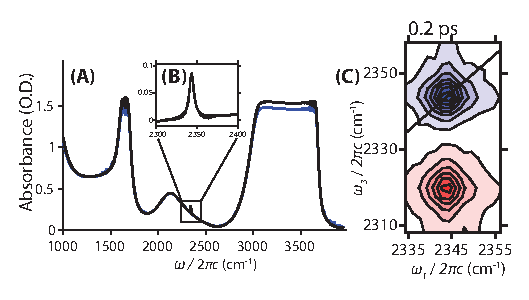
\includegraphics[scale=1.25]{./paper_01/fig1.eps}
  \caption[Linear and 2D-IR of \texorpdfstring{\ce{CO2} in \ce{H2O}}{carbon dioxide in water}]{\label{fig:CO2 in water}(A) FTIR spectrum of \ce{H2O} with (blue line) and without (black line) \ce{CO2} dissolved in it. \ce{CO2} \(\nu_3\) lies in the overtones and combinations bands from \ce{H2O} librational modes. (B) Inset of \(\nu_3\) with water background subtracted shows the Lorentzian character of the peak. (C) Purely absorptive 2D-IR spectrum of \(\nu_3\) in \ce{H2O} with \(t_2 = \SI{0.2}{\ps}\) shows that, in water, the line is nearly completely in the limit of homogeneous dynamics.}
\end{figure}

The other vibrational modes of \ce{CO2}, the symmetric stretch, \(\nu_1\), and the doubly degenerate bend, \(\nu_2\) and \(\bar{\nu}_2\), present distinct challenges for vibrational spectroscopy. The \(\nu_2\) modes are sensitive to the chemical environment of the \ce{CO2},\cite{Meredith1996,Kazarian2000} but are located in the crowded fingerprint region. The Raman active \(\nu_1\) is readily measured, but the lineshape is dominated by the Fermi resonance with the overtone of the \(\nu_2\);\cite{Cabaco2011} furthermore, it is a dark mode for IR.

Here, we demonstrate that the \ce{CO2} \(\nu_3\) mode reports on its local solvent environment by showing the sensitivity of the \(\nu_3\) frequency and dynamics to variation in solvent anion in a series of imidazolium ionic liquids; furthermore, we show that \(\nu_3\) reports a broad range of solvation timescales in these ionic liquids. We employ electronic structure calculations to investigate the mapping of vibrational frequencies onto structures of \ce{CO2}-anion-cation clusters. We show that, despite apparent complexity, the \ce{CO2} linear and 2D-IR lineshapes can be interpreted using simple and accurate physical models. Finally, we establish correlations between the measured dynamics of \ce{CO2} and the macroscopic properties of its ionic liquid solvent.

The paper is organized as follows. Initially, we present the analysis and interpretation of the linear \ce{CO2} spectrum (Section~\ref{sec:anions_linear}), including a discussion of its temperature dependence. Next, we describe the our results from electronic structure calculations on \ce{CO2}-anion-cation clusters and its relationship to our experimental data (Section~\ref{sec:vib_calcs}), followed by a simple model of \ce{CO2} that is able to reproduce the observed trends (Section~\ref{sec:freq-geom_disc}). We then present an overview of the 2D-IR spectra (Section~\ref{sec:anions_2DIR}), including a kinetic analysis of the observed shoulders and cross-peaks (Section~{\ref{sec:shoulders}), assignments of the spectral features (Section~\ref{sec:nu3_assignment}), and modelling of the main \(\nu_3\) peak (Section~\ref{sec:anions_2DIR_analysis}) and shoulders and cross-peaks (Section~\ref{sec:shoulders_modeling}). Finally, we present a discussion of the physical interpretation of our results (Section~\ref{sec:anions_interpretation}), conclusions (Section~\ref{sec:anions_conclusions}) and methods (Section~\ref{sec:anions_methods}).

\section{\texorpdfstring{\caps{Methods}}{Methods}}
\label{sec:anions_methods}

\subsection{Materials}
\label{sec:anions_methods_materials}

Ionic liquids were obtained from Ionic Liquids Technologies, Inc (IoLiTec), and used without further purification (except for \ce{[Im_{4,1}][BF4]}, which was purified prior to experiments using the procedure described by Giernoth and Bankmann.\cite{Giernoth2008}) Ionic liquid samples were stored in ambient conditions; however, prior to experiments, samples dried under vacuum at \SI{50}{\milli\torr}.

\subsection{FTIR}
\label{sec:anions_methods_ftir}

FTIR spectra were measured using a \ce{N2_{(g)}}-purged Nicolet 6700 FTIR instrument (ThermoFisher Scientific). Ionic liquid samples were loaded with \ce{CO2} (99.8\% purity, Matheson TRIGAS) in an airtight custom glass vial, with a septum that allows access to the \ce{CO2}-loaded ionic liquid. An aliquot of the liquid sample was sandwiched between two 2~mm-thick \ce{CaF2} optical windows (Crystran Ltd, UK) separated by a \SI{25}{\micron} Teflon spacer, which were held in a brass sample cell. The cell was assembled in a glove bag to limit adsorption of atmospheric water. Spectra were obtained for both the neat ionic liquid and for the ionic liquid loaded with \ce{CO2}.

For temperature-dependent measurements, the sample was temperature-controlled by using a cooling/heating recirculating chiller (Fisher Isotemp) to control the temperature of the sample cell holder. The sample temperature was monitored by measuring the temperature at the optical window using a thermocouple (National Instruments USB-TC01 J-type).

\subsection{2D-IR}
\label{sec:anions_methods_tdir}

\subsubsection{Generation of femtosecond mid-IR pulses}
\label{sec:anions_methods_tdir_generation}

The experiments utilize a commercial Ti:Sapphire chirped pulse amplifier laser system (\(\lambda = \SI{805}{\nm}\), \SI{5}{\kilo\hertz} repetition rate, \SI{120}{\fs} pulse duration) (Coherent Vitesse / Coherent Legend Elite).

A home-built optical parametric amplifier (OPA) generates the mid-IR pulses (\(\lambda = \SIrange{12}{2}{\micron}\)), corresponding to around \SIrange{830}{5000}{\wavenumber}. The OPA design leads to noise suppression in the resulting mid-IR pulses.\cite{Hamm2000} The spectral bandwidth after the OPA is about \SI{200}{\wavenumber}. For these experiments, we tune the OPA wavelength to \SI{4.3}{\micron}. Mid-IR pulse energy entering the 2D spectrometer is approximately \SI{2.2}{\micro\joule} per pulse.

\subsubsection{2D Spectrometer}
\label{sec:anions_methods_tdir_spectrometer}

The 2D-IR spectrometer uses a pump-probe geometry,\cite{Helbing2010} in which the first two mid-IR pulses travel collinearly to the sample. A Mach-Zehnder interferometer controls the coherence time \(t_1\) between these pulses. A delay stage after the interferometer controls the population time \(t_2\) between the second and third pulses. The signal, which contains both rephasing and non-rephasing components, is emitted in the direction of the probe pulse (\(\vec{k}_3\)), which also serves as a local oscillator to heterodyne the signal.

A 150 line/mm grating in a single monochromator disperses the signal in \(\omega_3\) onto a liquid \ce{N2}-cooled \(2 \times 32\) channel mercury cadmium telluride (MCT) detector. The signal in \(\omega_1\) is indirectly acquired by scanning along \(t_1\) using the Mach-Zehnder interferometer, and then applying a numerical Fourier transform to the resulting \(t_1\)-dependent signal at each data point in \(\omega_3\) (which also removes the transient absorption signal). The delay changes as the interferometer scans along \(t_1\) are acquired by comparing the interference pattern generated by a He:Ne beam which travels a parallel path through the interferometer.

A series of spectra in \(t_2\) are then acquired by varying the population time between the second and third laser pulses, and then obtaining a spectrum in \(\omega_1\) and \(\omega_3\) at each population time.

\subsection{Global Fitting and Bootstrapping}
\label{sec:anions_methods_fitting}

Global fitting of spectra utilizes a third-order response function formalism in the semi-impulsive limit, including the Condon approximation and also the approximation of the cumulant expansion truncated after second order. A constrained nonlinear optimization algorithm (\verb!fmincon! MATLAB) is used to minimize the magnitude of the sum of squared error between each data point in the set of spectra and a corresponding data point in a calculated spectrum. A bootstrapping algorithm \cite{numericalrecipes-92} establishes the error of the global fitting result. The global fitting algorithm was run using synthetic data sets composed of a random selection of the original data points taken with replacement. The distribution of the fitting parameters after 100 iterations provided the error estimate.

\subsection{Computational Details}
\label{sec:anions_methods_computational}

All calculations were performed with a development version of the Q-Chem program package\cite{Shao2015}, employing the B3LYP density functional, the 6-31G(d,p) basis set, and a (100,302) grid for the numerical quadrature. All SCF calculations were tightly converged to below \num{e-9}~a.u.\ for the DIIS error. Gas-phase geometry optimizations of free \ce{CO2} and the \ce{CO2}--ionic liquid clusters were converged to changes of \num{1d-8}~a.u.\ in the energy, \num{1d-6}~a.u.\ in the nuclear displacement, and \num{1d-6}~a.u.\ in the gradient. Optimized structures were confirmed as minima via harmonic frequency calculations using analytic Hessians. Frequencies were scaled by a factor of \num{0.9627} (Table 6 Merrick et al.)\cite{Merrick2007}.

For the calculations including the electrostatic and polarization effects of the ionic liquid with charge transfer disabled (``\(+ \Delta \omega_\mathrm{FRZ} + \Delta \omega_\mathrm{POL}\)'' in Figure~\ref{fig:decomposition}), absolutely localized molecular orbitals (ALMOs)\cite{Khaliullin2006} were employed, with the ionic liquid constituents as one combined fragment and the \ce{CO2} as another fragment. Solution of the ALMO equations is requested by setting \verb!frgm_method = gia!. Charge transfer between fragments is disabled by setting \verb!frgm_lpcorr = 0!. For the calculation of complementary occupied-virtual pairs (COVPs), an energy decomposition analysis (ALMO-EDA) calculation is performed where charge transfer is allowed (\verb!frgm_lpcorr = rs_exact_scf!).

\section{\texorpdfstring{\caps{Results and Discussion}}{Results and Discussion}}

\subsection{Linear IR Spectroscopy Results}
\label{sec:anions_linear}

The linear spectra of \ce{CO2} establish that the \(\nu_3\) mode is sensitive to the anion, and set the stage for discussing the spectroscopic features present in the 2D-IR spectra.

The \(\nu_3\) vibration absorbs strongly around \SI{2340}{\wavenumber} in a spectral region with no strong solvent absorbances (Figure~\ref{fig:FTIR}A). The lineshape of the \(\nu_3\) band (Figure~\ref{fig:FTIR}B) appears mostly Lorentzian, with a low frequency shoulder.
\begin{figure}
  \centering
  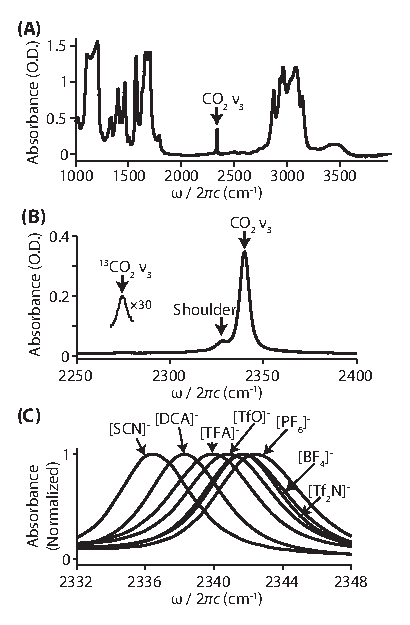
\includegraphics[scale=1.40]{./paper_01/fig2.eps}
  \caption[FTIR of \texorpdfstring{\ce{CO2}}{carbon dioxide} in ionic liquids]{\label{fig:FTIR} a) Absorption spectrum of \ce{CO2} in \ce{[Im_{4,1}]}[TFA] shows the intense antisymmetric stretch absorption at \SI{2340}{\wavenumber}; b) the background subtracted spectrum is Lorentzian with a shoulder at \SI{2328}{\wavenumber}, the \(\nu_3\) band of the \ce{^{13}C} isotopomer is located at \SI{2280}{\wavenumber}; c) The average vibrational frequency of the \(\nu_3\) absorption of \ce{CO2} shifts for different anions and the same \ce{[Im_{4,1}^+]} cation (background subtracted).}
\end{figure}

Changing the anion causes both the full-width at half-maximum (FWHM) and center frequency of \(\nu_3\) to change (Figure~\ref{fig:FTIR}C). We varied the anion, rather than the cation, because the anion dominates \ce{CO2} solubility in ionic liquids.\cite{anthonyJPCB-05,Cadena2004,Bhargava2007} Anions studied were hexafluorophosphate (\ce{PF6-}), tetrafluoroborate (\ce{BF4-}), bis-(trifluoromethyl\-sulfonyl)imide (\ce{Tf2N-}), triflate (\ce{TfO-}), trifluoroacetate (\ce{TFA-}), dicyanamide (\ce{DCA-}), and thiocyanate (\ce{SCN-}). The cation in all experiments was 1-butyl-3-methylimidazolium (\ce{[Im_{4,1}]}).

The \(\nu_3\) center frequency progressively redshifts from a maximum of \SI{2342.5}{\wavenumber} (\ce{[PF6-]}) to a minimum of \SI{2336}{\wavenumber} (\ce{[SCN]-}). The shoulder moves with the main absorption band and stays \(\sim\SI{12}{\wavenumber}\) lower in frequency.  Qualitatively, smaller, harder anions like \ce{[SCN]-} and \ce{[DCA]-} create a larger redshift than bulkier, softer anions like \ce{[Tf2N]-} and \ce{[TfO]-}, which is most likely a function of increased anionic charge density. The increased charge density could red-shift the \ce{CO2} center frequency though an increased local electric field (Stark effect), through charge transfer, or through inductive effects. Quantum chemistry calculations (Section~\ref{sec:vib_calcs}) help to disentangle the driving forces behind this qualitative trend.

The shoulder on the low frequency side of the main \(\nu_3\) transition could arise from several possible mechanisms, a ``hot-band'', a multiple-quantum transition, or different chemical environments. The temperature dependence of this feature is important in discriminating among these possibilities.

Temperature-dependent FTIR demonstrates that the shoulder on the low frequency side of the main \(\nu_3\) transition  is a hot band of the \(\nu_3\) mode (Figure~\ref{fig:hot band}A). Increasing temperature causes a decrease in intensity of the main peak and an increase in intensity of the shoulder, while conserving oscillator strength. The relative magnitude of the shoulder (\(\sim 10\%\) of the main band at room temperature) is similar to the expected relative excited state bending mode (\(\nu_2\)) population predicted by a Boltzmann distribution.

\begin{figure}
  \centering
  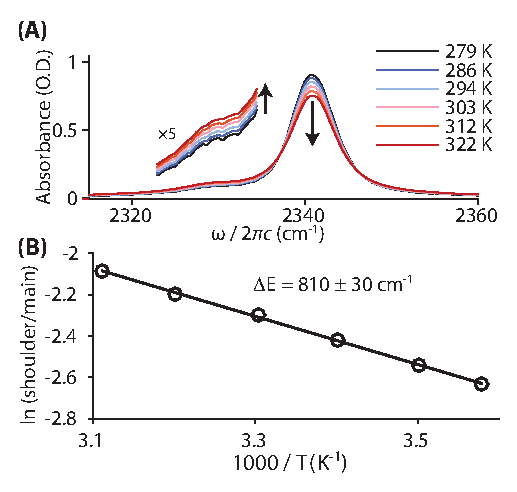
\includegraphics[scale=1.40]{./paper_01/fig3.eps}
  \caption[T-dependent FTIR of \texorpdfstring{\ce{CO2}}{carbon dioxide} in 1-butyl-3-methylimidazolium triflate]{\label{fig:hot band}(A) Temperature dependence of the \(\nu_3\) spectrum in \ce{[Im_{4,1}]}[TfO] shows transition of intensity from the main peak to the shoulder with increasing temperature, indicating a temperature-dependent two-state transition. (B) Relative intensity of shoulder to the main band (based on fitting to Voigt profiles) follows a van't Hoff temperature dependence, indicating an energy barrier of around \SI{800}{\wavenumber}, which closely follows the prediction from the temperature dependence of bending mode population.}
\end{figure}

We fit the spectra in Figure~\ref{fig:hot band}A to two Voigt profiles (one for the main peak, and one for the first shoulder seen on the 2D-IR).

A van't Hoff analysis of the logarithm of the relative peak heights against \(1/T\) gives an activation energy of \SI{810(30)}{\wavenumber}. This value is near the energy of the \(\nu_2\) bending vibration (\SI{667}{\wavenumber}). Residual gas lines and nonlinearity of the detector contribute to the systematic error of this measurement. Nevertheless, the temperature dependence strongly suggests that the first shoulder is due to one quantum of the bending mode which is excited thermally and is anharmonically coupled to the \(\nu_3\) mode.

The temperature dependence and hot-band assignment are important components of our interpretation of the shape of the 2D-IR spectra (Section~\ref{sec:shoulders}) and their time-dependence (Section~\ref{sec:shoulders_modeling}).

\subsection{Vibrational Frequency Calculations}
\label{sec:vib_calcs}

Electronic structure calculations provide a rationale for the observed trend in vibrational frequencies.

Harmonic frequency calculations reproduce the general trend that \(\nu_3\) progressively redshifts with decreasing anion size (Table \ref{tab:1}).  We simplify the solvated \ce{CO2} structure to a gas-phase cluster consisting of one \ce{CO2} with one cation-anion pair, with 1,3-dimethylimidazolium (\ce{Im_{1,1}}) as the cation. When scaled with the appropriate factor\cite{Merrick2007}, the simulations calculate vibrational frequencies within a few wavenumbers of the experimental value. The ordering of anions mostly agrees with experiment as well, the only outliers being \ce{[TFA]-} and \ce{[SCN]-}, which are located only \SI{2.3}{\wavenumber} apart.

The level of agreement between experiment and theory is good, given that the condensed phase environment is neglected. That such a simple representation reproduces the general trends so well suggests that the interactions of \ce{CO2} are dominated by local effects in its immediate surroundings. Future work will address the condensed phase effects by sampling representative structures from molecular dynamics simulations and repeating the analysis in the context of larger solvation shells.

Encouraged by the fact that the electronic structure calculations reproduce the experimental trends in \(\nu_3\) frequencies, we decompose the calculated vibrational frequencies into different components using absolutely localized molecular orbitals (ALMO), in analogy to ALMO energy decomposition analysis (ALMO-EDA).\cite{Khaliullin2006,Khaliullin2007,Khaliullin2008}

Unlike standard quantum chemical calculations, where individual molecular orbitals may delocalize over more than a single fragment, each ALMO is composed of atomic orbitals from a single fragment. This constraint allows us to control charge transfer between fragments and to quantify the interaction between fragments in physically intuitive terms.

The total vibrational frequencies \(\omega_{\mathrm{tot}}\) and vibrational shifts \(\Delta \omega_\mathrm{int}\) from gas phase (``free'') \ce{CO2} for each mode \(\nu\) may be written as:
\begin{equation}
  \omega_\mathrm{tot} = \omega_\mathrm{free} + \Delta \omega_\mathrm{int}
\end{equation}
where
\begin{equation}
  \Delta \omega_\mathrm{int} = \Delta \omega_\mathrm{GEOM} + \Delta \omega_\mathrm{FRZ} + \Delta \omega_\mathrm{POL} + \Delta \omega_\mathrm{CT}
\end{equation}
where \(\Delta \omega_\mathrm{GEOM}\) (geometric distortion) corresponds to the change in frequency caused by distortion of fragments from their free geometries to their cluster geometries, \(\Delta \omega_\mathrm{FRZ}\) (the frozen orbital interaction) results from the combined electrostatic interaction and Pauli repulsion between the filled, unrelaxed orbitals of each fragment, \(\Delta \omega_\mathrm{POL}\) (polarization) is due to the relaxation of a fragment's orbitals in the field of the other fragments, and \(\Delta \omega_\mathrm{CT}\) (charge transfer) is from occupied-virtual orbital donation between orbitals of different fragments.\cite{Ramos-Cordoba2011}

The cluster environment can affect the vibrational frequency of \ce{CO2} in two different ways. The first depends on the anharmonic potential surface of a free \ce{CO2} molecule. In a harmonic system, the spring constant, \(k\), uniquely determines the vibrational frequency for all nuclear positions (i.e., the curvature of a quadratic potential is constant). \ce{CO2}'s potential energy surface, however, is inherently anharmonic. Any change in geometry will thus cause a change in the \(\nu_3\) vibrational frequency. In other words, the cluster can change the \(\nu_3\) frequency just by shifting the location of minimum of the \ce{CO2} potential (\(\Delta \omega_\mathrm{GEOM}\)). The second results from changes in the local curvature of \ce{CO2}'s potential energy surface due to interactions with the surrounding cluster (\(\Delta \omega_\mathrm{FRZ} + \Delta\omega_\mathrm{POL} + \Delta \omega_\mathrm{CT}\)).

We focus on the following grouping of terms: (1) distortion of isolated \ce{CO2} to its cluster geometry (\(\Delta \omega_\mathrm{GEOM}\)), (2) the combined frozen orbital and polarization contributions through use of ALMOs (\(\Delta \omega_\mathrm{FRZ} + \Delta \omega_\mathrm{POL}\)), and (3) charge transfer between the fragments in the cluster (\(\Delta \omega_\mathrm{CT}\)).

The final frequency, \(\omega_\mathrm{tot}\), correlates most strongly with \(\Delta \omega_\mathrm{GEOM}\) (\(R^2 = 0.96\)), indicating that geometrical distortion of \ce{CO2} dominates the frequency shift. Depending on the particular geometry that \ce{CO2} adopts in the cluster, \(\Delta \omega_\mathrm{GEOM}\) can vary by \SI{\pm 6}{\wavenumber} (Figure~\ref{fig:decomposition}).\footnote{Since \(\omega\) normally refers to an angular frequency, this quantity might more rigorously be be called \(\Delta \omega_\mathrm{GEOM} / 2 \pi c\); however, for convenience of notation, we chose to use spectroscopic units uniformly in this section. That is, all frequencies are given in wavenumbers, rather than \si{\radian\per\second}.} Electrostatics and charge transfer both change the local curvature of the potential energy surface; however, their effects are mostly uniform across the ionic liquids studied. When we turn off charge transfer between fragments, \(\nu_3\) blue-shifts on average by \(\braket{\Delta \omega_\mathrm{FRZ} + \Delta \omega_\mathrm{POL}} = \SI{+2.8(6)}{\wavenumber}\). Modelling the cluster geometry as a field of point charges increases this blue shift to \SI{+4.4(6)}{\wavenumber} (Supplementary Information), which may indicate that a point-charge representation of the cluster over-polarizes the QM region~\cite{Bakowies1996,Hu2011} Allowing charge transfer red-shifts the frequencies by \(\braket{\Delta \omega_\mathrm{CT}} = \SI{-3.5(8)}{\wavenumber}\).  Thus, both electrostatics and charge transfer change the local curvature of the \(\nu_3\) potential energy surface. The effects, however, are uniform and nearly cancel. The net result is that the inherent anharmonicity of the \ce{CO2} potential energy surface ultimately dominates the \(\nu_3\) frequency.

The geometrical distortion of the \ce{CO2} is driven by charge transfer. Using ALMOs and forbidding charge transfer during relaxation of the cluster removes the variance in \(\Delta \omega_\mathrm{GEOM}\) (Figure~\ref{fig:decomposition}B). Once again, both electrostatic and charge transfer interactions act uniformly on the frequency, leading to a negligible variance in \(\omega_\mathrm{tot}\). Without the geometrical distortion due to charge transfer, the vibrational frequencies for all clusters remain within $\pm2$~\si{\wavenumber} and no longer follow the experimental trend.

The essential point is that charge transfer and electrostatics only affect the vibrational frequency indirectly, through their coupling into the equilibrium \ce{CO2} nuclear geometry. The direct effects of electrostatics and charge transfer on the potential energy surface (and thus the effective spring constant) of \(\nu_3\) are uniform across ionic liquids studied and counteract each other.

This DFT-based analysis may over-emphasize charge transfer to some extent. It is well known that DFT over-delocalizes electrons due to self-interaction error, which might exaggerate the amount of charge transfer. In the context of gas-phase anion clusters, both DFT\cite{breen-JPCA12} and post-Hartree-Fock methods\cite{Muraoka2009} have also identified charge transfer as a driver of geometrical distortion of \ce{CO2}, so we expect that our qualitative picture will be robust with respect to the theoretical method. Future work will explore the quantitative differences between the different methods. Furthermore, although our cluster results agree well with experiment, we expect that the extended solvation environment neglected here may introduce screening effects not captured at the cluster level.\cite{Lee2011a}  A more sophisticated study of solvation effects could determine whether our finding, that charge transfer dominates the geometric effects which differentiate \ce{CO2} vibrational frequency shifts, is transferable to bulk ionic liquids.

These calculations demonstrate that the \(\nu_3\) frequency shift reflects a complex interplay between geometry, electrostatics, and charge transfer. The geometrical distortion is the most important factor in determining the final variation in vibrational frequency with anion identity; however, the equilibrium geometry of the \ce{CO2} itself ultimately depends on inductive effects, such as charge transfer.

\begin{table}
  \centering
  \caption[Experimental and calculated \texorpdfstring{\ce{CO2} \(\nu_3\)}{carbon dioxide antisymmetric stretch} vibrational frequencies]{\label{tab:1}Experimental and calculated \(\nu_3\) vibrational frequencies for \ce{CO2} in various imidazolium (experimental \ce{[Im_{4,1}]}, calculations [\ce{Im_{1,1}}]) ionic liquids. Calculations are carried out using a gas phase anion-cation-\ce{CO2} cluster at 0 K. The level of agreement between calculations and experimental results indicates that interactions of \ce{CO2} are dominated by local effects in its immediate surroundings.}
  \begin{tabular}{cccc}
    \toprule
    Anion & Expt. Freq. & Calc.\ Freq. & Calc.\ Freq. (scaled) \\
          & (\si{\wavenumber}) & (\si{\wavenumber}) & (\si{\wavenumber}) \\
    \midrule
    \ce{[PF6]-} & 2342.5 & 2437.7 & 2346.8 \\
    \ce{[Tf2N]-} & 2341.7 & 2435.8 &2344.9 \\
    \ce{[BF4]-} & 2341.7 & 2434.7 & 2343.9 \\
    \ce{[TfO]-} & 2340.9 & 2431.9 & 2341.2 \\
    \ce{[TFA]-} & 2339.9 & 2429.3 & 2338.7 \\
    \ce{[DCA]-} & 2338.4 & 2430.5 & 2339.8 \\
    \ce{[SCN]-} & 2336.5 & 2430.0 & 2339.4 \\
    \bottomrule
  \end{tabular}
\end{table}

\begin{figure}
  \centering
  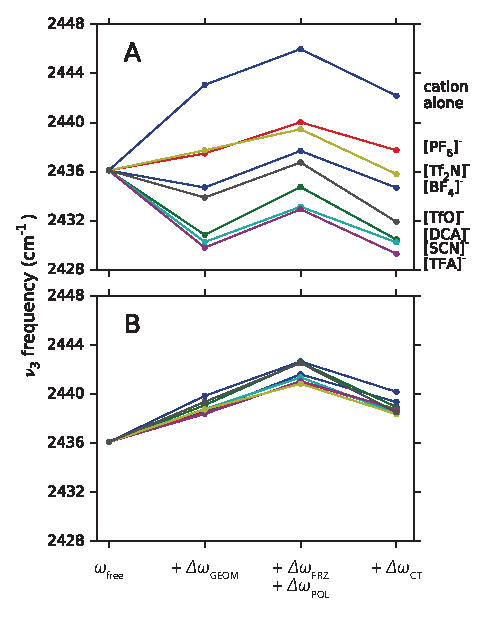
\includegraphics[scale=1.50]{./paper_01/fig4.eps}
  \caption[ALMO decomposition of \texorpdfstring{\ce{CO2} \(\nu_3\)}{carbon dioxide asymmetric stretch} frequency]{\label{fig:decomposition}Decomposition of the geometric, electrostatic, and charge transfer contributions to \ce{CO2} \(\nu_3\) vibrational frequency shifts. (A) The cluster geometry (including \ce{CO2}) was optimized while allowing charge transfer. (B) The cluster geometry was optimized using ALMOs to forbid charge transfer between fragments. The final frequency (\(\omega_\mathrm{tot} = \omega_\mathrm{free} + \Delta \omega_\mathrm{GEOM} + \Delta \omega_\mathrm{FRZ} + \Delta \omega_\mathrm{POL} + \Delta \omega_\mathrm{CT}\)) correlates most strongly with the change in frequency from geometric distortion (\(\Delta \omega_\mathrm{GEOM}\)).}
\end{figure}

\subsection{Frequency, Geometry, and  Charge Transfer Discussion}
\label{sec:freq-geom_disc}

To gain chemical insight into the charge transfer process, one can analyze the donor and acceptor orbitals of \ce{CO2} and the ionic liquid. This analysis sheds light on the nature of the geometrical distortion, which, in turn, leads to a simple model for the vibrational frequencies in terms of a few geometrical parameters.

We employ a complementary occupied-virtual orbital pair (COVP) analysis\cite{Khaliullin2008} to gain insight into the electronic structure effects underlying the charge transfer between \ce{CO2} and the solvent. COVPs provide a way to visualize charge transfer effects, where ``each COVP corresponds to an occupied orbital on one molecule donating charge to one specific (complementary) virtual orbital on the other molecule.''\cite{Khaliullin2009} These orbital pairs are constructed from a singular value decomposition of the occupied-virtual mixing matrix \(\mathbf{X}\) that describes charge transfer between the (polarized) fragments upon removing the ALMO fragment localization constraint. While \(\mathbf{X}\) contains, in general, excitations between all possible occupied-virtual pairs, the COVP representation of \(\mathbf{X}\) is diagonal and thus provides the most compact possible basis for describing charge transfer.  The associated singular values allow one to assess the contribution of a particular COVP to charge transfer, and typically one finds that only one or a few orbital pairs dominate the effect (as shown below in this study). The COVP analysis thus allows to conveniently identify and visualize the electron donor/acceptor orbitals pair(s) that significantly contribute to charge transfer.

Charge transfer to the \ce{CO2} originates from occupied orbitals on the anions. The charge is accepted by virtual orbitals on the \ce{CO2}. The virtual orbitals are a linear combination of the LUMO and LUMO+1 orbitals, which have \(\sigma^{*}\) and \(\pi^{*}\) character, respectively. Charge transfer from the anion has a strong linear correlation to the bend angle (\(R^2=0.84\)). Mechanistically, bending the \ce{CO2} allows \(\sigma^{*}\) and \(\pi^{*}\) to mix, lowers the energy of the acceptor orbital, and also maximizes the spatial overlap with the donor orbital. The amount of charge transferred (\SIrange{3}{5}{\milli\electron}) is small, but the resulting bend angle (\SIrange{3}{5}{\angstrom}) can be substantial (Table~\ref{tab:ct}).
\begin{table}
  \centering
  \caption[\texorpdfstring{\ce{CO2}}{Carbon dioxide} geometry dependence on charge transfer]{\label{tab:ct}Charge transfer from the anion to \ce{CO2} and from \ce{CO2} to the cation both contribute to the geometrical distortion of the \ce{CO2}. The most important geometrical degrees of freedom are the bend angle, \(\theta\) and the sum of the two carbonyl bond lengths, \(L\).}
  \begin{tabular}{ccccc}
    \toprule
    cluster & CT to \ce{CO2} (\si{\milli\electron}) & CT from \ce{CO2} (\si{\milli\electron}) & \(\theta\) (\si{\degree}) & \(L\) (\si{\angstrom}) \\
    \midrule
    \ce{[Im_{1,1}]+} & 0.079 & 2.251 & 0.07 & 2.3374 \\
    \ce{[PF6]-} & 3.336 & 1.012 & 3.79 & 2.3379 \\
    \ce{[Tf2N]-} & 2.493 & 1.603 & 2.64 & 2.3380 \\
    \ce{[BF4]-} & 4.558 & 1.264 & 4.51 & 2.3385 \\
    \ce{[TfO]-} & 3.009 & 2.339 & 4.01 & 2.3389 \\
    \ce{[TFA]-} & 5.131 & 1.618 & 5.22 & 2.3394 \\
    \ce{[DCA]-} & 3.376 & 2.259 & 4.99 & 2.3394 \\
    \ce{[SCN]-} & 3.317 & 1.323 & 4.35 & 2.3395 \\
    \bottomrule
  \end{tabular}
\end{table}

\ce{CO2} also donates charge back to the ionic liquid cluster, primarily to the cation. The amount of charge donated by the \ce{CO2} to the cation (\SIrange{-1}{-2}{\milli\elementarycharge}) is typically less than the charge donated from the anion, but nevertheless has specific consequences for the resulting geometry. The donor orbital from the \ce{CO2} is a mixture of \(\sigma\)-bonding and \(\pi\)-nonbonding character. The charge donation from the \ce{CO2} is linearly correlated to the carbonyl bond length differences (\(R^2 = 0.85\)). For the \ce{[Im_{1,1}][TfO]} cluster, which has the highest charge transfer from \ce{CO2} to the cation (\SI{2.32}{\milli\electron}), the \(\sigma\) character of the donating orbital causes the carbonyl nearest the cation to lengthen from the gas-phase \SI{1.169}{\angstrom} to \SI{1.175}{\angstrom} while the distal carbonyl contracts to \SI{1.163}{\angstrom}.

The effects of charge transfer to and from the \ce{CO2} can be incorporated into a simple model of the vibrational frequencies. The model is constructed in a vibrational local-mode basis. The effective one exciton vibrational Hamiltonian is

\begin{equation}
  H^{(1)} =
  \begin{pmatrix}
    \hbar\omega_1 & \beta\\
    \beta & \hbar\omega_2
  \end{pmatrix}
\end{equation}
where \(\omega_i\) is the local mode frequency of carbonyl \(i\) and \(\beta\) is the coupling between the two local modes. The diagonalized hamiltonian gives symmetric and antisymmetric linear combinations of the local modes as the vibrational eigenstates with energies \(\hbar\omega_s\) and \(\hbar\omega_a\). The splitting between symmetric and antisymmetric vibrations is twice the coupling constant, \(\hbar(\omega_s - \omega_a) = 2\beta\), and the average frequencies in local and normal modes are also equal \(\hbar(\omega_a + \omega_s)/2 = \hbar(\omega_1 + \omega_2)/2 = \alpha\).

The bend in the \ce{CO2} determines the change in the coupling constant between the local modes, \(\beta\) (\(R^2 = 0.94\)). The motion of the central carbon atom is the primary motion that couples the two carbonyls. When they are collinear, the motion of one carbonyl directly influences the other. Bending the \ce{CO2} means the carbonyls are no longer collinear, which means that the projection of one local vibration on the other decreases. This decrease, in turn, decreases the effective coupling constant.

The sum of the \ce{CO2} bond lengths \(L\), is correlated to the \(\alpha\) (\(R^2 = 0.998\)). The dependence of \(\alpha\) on the geometry of the molecule is not as straightforward than that of \(\beta\). In the strong coupling limit, \(\beta \gg |\hbar\omega_2-\hbar\omega_1|\), the symmetric and antisymmetric stretching frequencies only depend on the average frequencies, \((\hbar\omega_1 + \hbar\omega_2)/2\). As such, the geometrical asymmetry induced by charge transfer from the \ce{CO2}, which weakens one bond and strengthens the other, is largely averaged out. Only a weak correlation between the charge donated from the \ce{CO2} and the \(\alpha\) remains. The sum of the bond lengths, \(L\), however, reports exactly this difference in total bonding strength. Though the changes in \(L\) are minute (\(\sim \SI{0.001}{\angstrom}\)), the effect on the vibrational frequencies is not.

Because of the strong linear correlation with these two geometrical variables, we propose that the simplest model of the scaled vibrational frequencies is \(\alpha(L)\) and \(\beta(\theta)\), where
\begin{equation}
  \alpha(L) = \SI{9523.8}{\wavenumber} - \left(3415.3~\mathrm{cm}^{-1} \mathrm{\AA}^{-1}\right) L %scaled 0.9627
\end{equation}
and
\begin{equation}
  \beta(\theta) = \SI{-515.7}{\wavenumber} + \left(1.12~\mathrm{cm}^{-1} \mathrm{deg}^{-1}\right)\, \theta, %scaled 0.9627
\end{equation}
where \(\alpha\) and \(\beta\) are in units of \si{\wavenumber}, \(L\) is in \si{\angstrom}, and \(\theta\) is in degrees. The one exciton Hamiltonian
\begin{equation}
  H^{(1)} =
  \begin{pmatrix}
    \alpha(L) & \beta(\theta)\\
    \beta(\theta) & \alpha(L)
  \end{pmatrix},
\end{equation}
% TODO SI
reproduces the scaled harmonic frequencies with an RMS error of \SI{1.2}{\wavenumber} and the experimental frequencies with an RMS error of \SI{4}{\wavenumber}.\footnote{See section~\ref{paper_01:sec:SI} for 2D-IR spectra of \ce{CO2} in each ionic liquid, as well as a comparison of center line slope and global fitting results for correlation times, and more detailed computational results. Additionally, there is information on fitting of the one exciton Hamiltonian model for unscaled frequencies, and vibrational frequency calculations of \ce{CO2} in a field of point-charges that approximates the cluster geometry.}

Following a detailed investigation of the charge transfer, the participating orbitals, and the effects of charge transfer on the \ce{CO2} geometry, we have put forward a simple model that successfully reproduces the calculated vibrational frequencies and, to a reasonable extent, the experimental frequencies, with no free parameters.

\subsection{2D-IR Spectroscopy Overview}
\label{sec:anions_2DIR}

While linear spectroscopy shows the sensitivity of \ce{CO2} to its local environment, it cannot address the ultrafast dynamics of the chromophore. 2D-IR, however, directly reports on the dynamic structural relaxation around \ce{CO2}. 2D-IR of \ce{CO2} in \ce{[Im_{4,1}]}[TFA] introduces many of the features that are general across all of the ionic liquids studied.

The 2D spectra of the \(\nu_3\) mode of \ce{CO2} in \ce{[Im_{4,1}]}[TFA] (Figure~\ref{fig:example 2D}A and B) show the main \(\nu_3\) band, two diagonal shoulders, and cross-peaks between them. The observed peaks cannot be explained without also keeping track of the states of the \ce{CO2} symmetric stretch and bending modes in the vibrational state. The total vibrational wavefunction is specified by $|\nu_1 \nu_2^l \nu_3 \rangle$, where \(\nu_1\) is the number of quanta in the symmetric stretch, \(\nu_2\) is the number of quanta in the bending mode, $l$ is the vibrational angular momentum quantum number of the bending mode, and \(\nu_3\) is the number of quanta in the antisymmetric stretch.

The main band consists of a pair of intense peaks corresponding to the $|00^00\rangle\rightarrow|00^01\rangle$  and $|00^01\rangle\rightarrow|00^02\rangle$ (1a and 1b) transitions, separated by the anharmonicity of \(\nu_3\) (\(\sim \SI{24}{\wavenumber}\)). Due to ground state bleach, 1a appears as a negative (blue) feature, while 1b, from excited state absorption, is a positive (red) feature. The \(\nu_3\) shoulder appears as a pair of small peaks (2a and b), shifted along the diagonal by \SI{-12}{\wavenumber} in \(\omega_1\) and \(\omega_3\). A second apparent shoulder, not seen on FTIR, presents as a pair of smaller peaks (1e and 1f), shifted along the diagonal from the main band by \SI{-24}{\wavenumber} in \(\omega_1\) and \(\omega_3\). At early population times, there is an apparent cross-peak between the main peak and second shoulder (1c). Cross-peaks grow in between the first shoulder and main peak (2-1a and b, 1-2b) over \(t_2\). The expected cross-peak 1-2a cannot be seen due to cancellation with the overwhelming opposite signal from the 1b.

The combination of \ce{CO2}'s high molar absorptivity (\(\sim \SI{1000}{\per\Molar\wavenumber}\)) and the \(\varepsilon^2\) dependence of the third-order signal causes the 2D signal from \ce{CO2} to dominate the spectrum in intensity. Contributions from solvent overtones in the background are smaller than the level of noise in the spectrum. Thus, the 2D signal reflects the vibrational modes of \ce{CO2}, rather than solvent background, and the solvent can only affect the 2D spectrum through intermolecular couplings with \ce{CO2} vibrational modes.

\begin{figure}
  \centering
  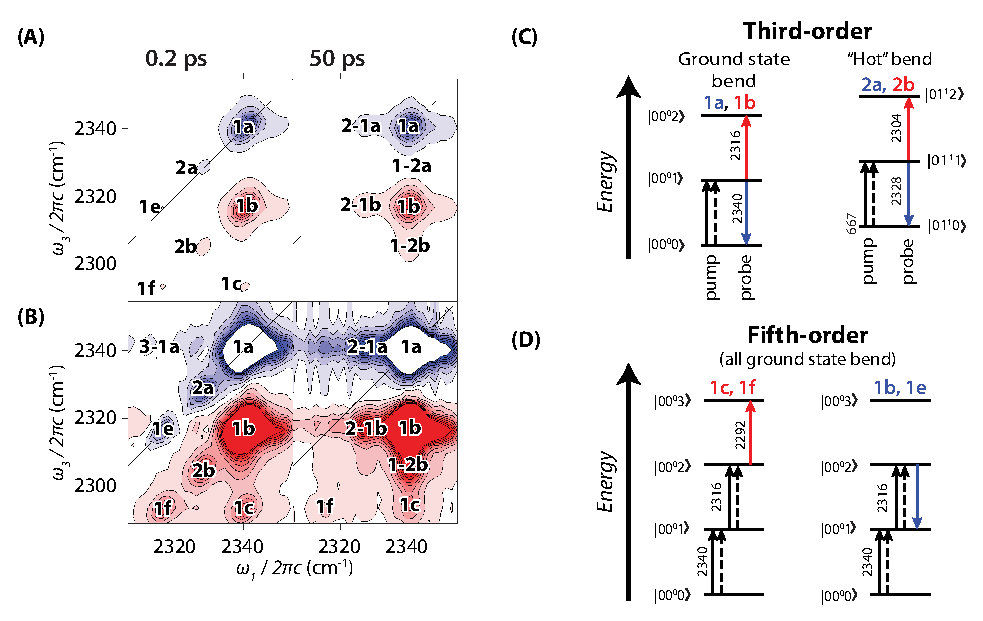
\includegraphics[scale=1]{./paper_01/fig5_update4.eps}
  \caption[2D-IR spectra of \texorpdfstring{\ce{CO2}}{carbon dioxide} in ionic liquids]{\label{fig:example 2D}\textbf{(A)} 2D-IR spectrum of \ce{CO2} in \ce{[Im_{4,1}][TFA]} at \(t_2\) = \SIlist[list-units = single]{0.2;50}{\ps}. The peak labels correspond to transitions in (C) and (D). \textbf{(B)} The same spectrum as (A) with contours limited to 10\% of the maximum in the $z$-direction. Structure of the diagonal shoulders and cross-peaks can be seen much more readily. \textbf{(C) and (D)} Vibrational energy level diagrams for observed third-order (C) and fifth-order (D) bands of \ce{CO2} in \ce{[Im_{4,1}][TFA]}. Quantum numbers correspond to $|\nu_1 \nu_2^l \nu_3\rangle$. Transition frequencies are labeled in wavenumbers (\si{\wavenumber}), and a label corresponding to the peaks in A and B. The color of the label indicates whether the expected peak is negative (blue) or positive (red).}
\end{figure}

The unambiguous spectral diffusion of 1a and 1b over the \SI{50}{\ps} population time demonstrates that the line is not entirely in the motional narrowing (homogeneous) limit. That is, \(\nu_3\) will allow us to resolve the dynamics of structural relaxation around \ce{CO2}.

The observations of a complex pattern of peaks and of spectral diffusion on a tens of picoseconds timescale for \ce{CO2} in \ce{[Im_{4,1}]}[TFA]  are general features of the spectra in all of the tested ionic liquids and are described in detail in the next two sections.

\subsection{2D-IR Shoulders and Cross-Peaks}
\label{sec:shoulders}

\begin{figure}
  \centering
  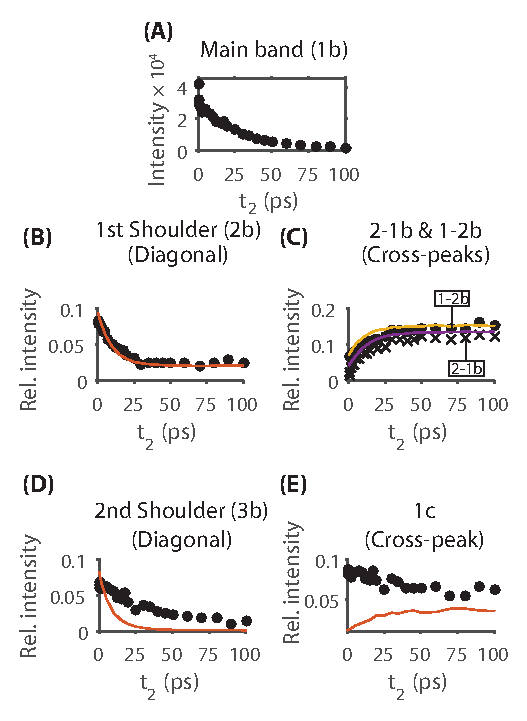
\includegraphics[scale=1]{./paper_01/fig6.eps}
  \caption[\texorpdfstring{\ce{CO2}}{Carbon dioxide} in IL bending mode kinetics]{\label{fig:shoulder kinetics}Kinetic analysis of \ce{[Im_{4,1}]}[TFA]. (A) Absolute intensity of the main peak (1b) with increasing \(t_2\). Decreased intensity results from both orientational and population relaxation. (B)-(E) show intensities relative to A. Discrete data points represent experimental data, while lines show data from stochastic simulations (Section~\ref{sec:shoulders_modeling}). (B) and (C), which result from the first diagonal shoulder (2b) and its cross-peaks with the main band (1-2b / 2-1b) show good agreement between experimental and simulated kinetics. (D) and (E), which result from the second diagonal shoulder (3b) and the apparent cross-peak (1c) show distinct kinetics, which cannot result from the same stochastic bending mode fluctuations, and point to a direct transition.}
\end{figure}

Careful analysis of the relative kinetics of the diagonal peaks and cross-peaks (Figure~\ref{fig:shoulder kinetics}) provides insight into how the coupling of \ce{CO2} vibrational modes and their stochastic dynamics create the observed spectrum.

Orientational and vibrational relaxation of \ce{CO2} cause a decrease in spectral intensity over \(t_2\). The main peak (1b) shows an initial rapid decrease in intensity from orientation relaxation, followed by a slower decay over \(\sim \SI{100}{\ps}\), from vibrational relaxation processes. Polarization-controlled studies can remove the contribution from orientational relaxation, and provide an explicit assessment of vibrational relaxation rate.\cite{hamm_concepts_2011,Hochstrasser2001}

The shoulders and cross-peaks are significantly weaker than the main peak, and also relax over \(t_2\); however, analysis of their kinetics relative to the main band reveals the underlying stochastic dynamics of \ce{CO2} vibrational modes.

The first diagonal shoulder (2b) decays more quickly than the main band, decreasing to a minimum intensity at \(\sim \SI{25}{\ps}\) followed by a (relative) steady state (Figure~\ref{fig:shoulder kinetics}). Cross-peaks between the first shoulder and the main band (2-1b and 1-2b) start at a minimum intensity, and then increase, before reaching a relative steady state by 25 ps. This behavior points to dynamic exchange between \(|00^01\rangle\) and \(|01^11\rangle\), which give rise to the diagonal peaks (Section~\ref{sec:shoulders_modeling}).

The second diagonal shoulder (3b) decreases in intensity relative to the main band, but more slowly than the first shoulder. The apparent cross-peak 1c decreases in relative intensity over \(t_2\) with slower kinetics than the second shoulder. This behavior contrasts with that of the cross-peaks 1-2b and 2-1b, and indicates that 1c arises from a direct vibrational transition, rather than dynamic exchange.

\subsection{Peak Assignment}
\label{sec:nu3_assignment}
The Dunham expansion for anharmonically coupled vibrational modes provides a theoretical framework for building an analysis of coupled vibrational modes:
\begin{equation}
  \label{eq:Dunham expansion}
  E = \sum_{i} \hbar \omega_i \left( n_i + \frac{1}{2} \right) + \sum_{ij} x_{ij} \left( n_i + \frac{1}{2} \right) \left( n_j + \frac{1}{2} \right)
\end{equation}
where $\omega_i$ is the frequency of the mode, $n_i$ is the number of quanta in the mode, and $x_{ij}$ are anharmonic coupling constants. It directly follows that the energy of a particular mode is given by:
\begin{equation}
  \label{eq:anh_coupled_energy}
  \nu_{n_k \rightarrow n_k + 1} = \nu_k + 2n_{k}x_{kk} + \sum_{i \neq k} x_{ij}n_{i},
\end{equation}
which implies that transition energy will decrease by \(x_{ij}\) for every quantum of energy in an anharmonically coupled mode.\cite{Botan2008} Gas phase vibrational calculations predict \(x_{23} \approx \SI{-12}{\wavenumber}\) per quantum in \(\nu_2\).\cite{Taylor1993,Dressier1997}

The first shoulder can then be explained by anharmonic coupling of excited state bending modes with the asymmetric stretching mode. This coupling causes a frequency shift of \SI{-12}{\wavenumber}, and creates a shoulder on the linear and the 2D spectra (peaks 2a/2b on 2D-IR). Stochastic fluctuations in thermally populated bending modes cause dynamic 2D-IR cross-peaks.

This mechanism for dynamic cross-peaks is not unique to \ce{CO2} in ionic liquids; however, it is a nearly ideal system in which to observe and analyze it. The narrow total linewidth (\(\sim \SI{6}{\wavenumber}\)), combined with a large anharmonic coupling constant (\(x_{23} = \SI{-12}{\wavenumber}\)), leads to clear segregation of the resulting frequencies into distinct peaks. The difference in energy between the ground and first excited state \(\nu_2\) modes is only around \(3k_{\textrm{B}}T\), which is low enough to be thermally accessible, but high enough to be quantized. Finally, the rate of stochastic fluctuations in bending mode states is slow enough to preserve distinct diagonal bands at short population times, but fast enough to allow dynamic cross-peaks over the timescale of the experiment (\(\sim \SI{100}{\ps}\)).

Alternative hypotheses can be ruled out. There are two possibilities that need to be addressed. First, the shoulder is often assigned to a multiquantum transition. Second, the shoulder and cross-peaks could be due to chemical exchange.

The first \(\nu_3\) shoulder in our spectra is also present in the FTIR of \ce{CO2} dissolved in organic liquids and many polymers, and is often attributed to a multiquantum transition \(\nu_3 + \nu_2 - \nu_2\),\cite{Culp2010,Cunliffe-Jones1969,Kazarian1996,Meredith1996,Dobrowolski1992} where the difference in energy is attributed to splitting of normally degenerate \ce{CO2} \(\nu_2\) and \(\bar{\nu}_2\) bending modes. (This combination should perhaps be written as \(\nu_3 + \nu_2 - \bar{\nu}_2\) or \(\nu_3 + \bar{\nu}_2 - \nu_2\), but is typically presented without distinguishing between the two bending modes.) This hypothesis fails on several accounts. First, such a multiquantum transition is harmonically forbidden, so the transition dipole moment should be significantly lower than for the one quantum \(\nu_3\) transition. The intensity of the shoulder, however, directly follows a Boltzmann distribution for the \(\nu_2\) bending modes, which implies that the magnitude of the transition dipole moment is roughly equal for both the fundamental and this multiquantum transition.

Second, with this mechanism, a shoulder on the high frequency side of the fundamental should accompany the observed shoulder on the low frequency side. That is, there is no clear reason why the transition \(\nu_3 + \nu_2 - \bar{\nu}_2\), would be strongly allowed, but \(\nu_3 + \bar{\nu}_2 - \nu_2\) would not. Third, this hypothesis assumes that the splitting of the bending modes is an identical \SI{12}{\wavenumber}, but this is not the case.\cite{Kazarian2000}
Finally, in the 2D spectrum, this combination band would give rise to cross-peaks between the first shoulder and the main band (since each a \ce{CO2} molecule could undergo either transition with excitation), which would be present at the earliest population times, and would only relatively decay (rather than relatively increase) with \(t_2\). This behavior contradicts the observed spectral kinetics.

The temperature dependence of the shoulder (Figure~\ref{fig:hot band}) also excludes different chemical environments (such as multiple equilibrium geometries of a \ce{CO2}-anion interaction) undergoing chemical exchange. In this hypothesis, the most intense feature would be due to free \ce{CO2} and the shoulder to \ce{CO2} with a stronger chemical interaction. The growth of the cross-peaks would correspond to the exchange of these populations. However, the free \ce{CO2} band should be entropically favored and increase with increasing temperature while the shoulder should be enthalpically favored and decrease with increasing temperature. The opposite is observed, so this hypothesis can be ruled out. Additionally, the equal relative energy spacing of the diagonal shoulders from the main band for \ce{CO2} in every ionic liquid studied strongly suggests that the additional peaks arise from the \ce{CO2} itself, rather than from distinct chemical environments.

In contrast, the explanation of anharmonic coupling between \(\nu_2\) and \(\nu_3\) fits the temperature dependence, the transition dipole scaling, and accounts for the cross-peak kinetics. In our picture, each step requires only a one quantum transition for each peak, explains the presence of a shoulder on only one side of the fundamental, and correctly reproduces the cross-peak kinetics (over \(t_2\)) between the first shoulder and main band due to thermal excitation and de-excitation of the bend.

The apparent cross-peak 1c, as well as the second apparent shoulder (1e and 1f) are fifth-order signals, as can be shown by pump power-dependence, frequencies, and sign show that it is a fifth-order signal, as are several other features. Assignments of the \(\nu_3\) 2D-IR spectrum of carbon dioxide in 1-butyl-3-methylimidazolium trifluoroacetate \ce{[Im_{4,1}][TFA]}, are given in  Figure~\ref{fig:example 2D} and Table \ref{tab:fifth_order}).

The magnitude of third-order signal is linear in pump light intensity, since there are two pump electric field interactions, while that of fifth-order signal (with four electric field interactions) is quadratic. We assessed the magnitude of each peak when the pump power was changed by a factor of two (Table \ref{tab:fifth_order}). There is a clear distinction between the pump power dependence of the third order signals (1a, 1b, 2a, 2b, and their population exchange cross-peaks) and the fifth order signal (1c, 1e, 1f, and 31a). The reported intensity ratio is the ratio of volumes of a single peak when the pump power doubles. Thus, for the main `red' peak (1b: \(\nu_3\) excited state absorption with ground state \(\nu_2\)), peak volume goes up by a factor of \num{2.2 +- 0.1} when pump power doubles. Peak 1c's volume, however, increases by a factor of \num{3.3 +- 0.2}.
% TODO this bit here must come from the comment/erratum?
\begin{figure}
  \centering
  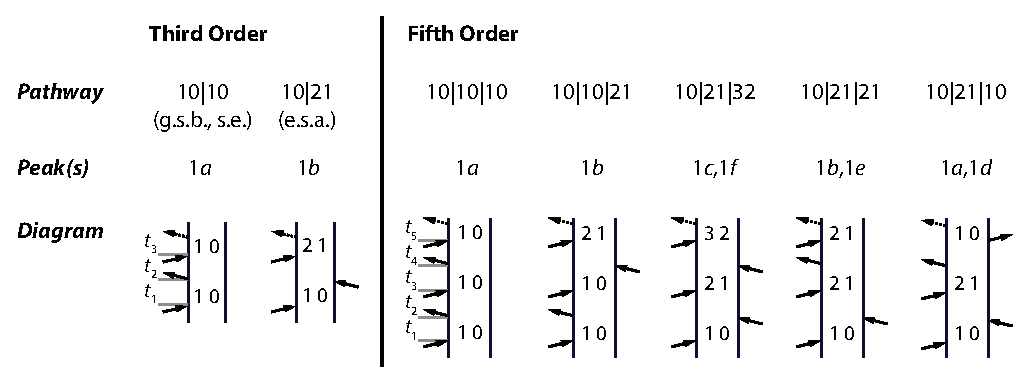
\includegraphics[scale=0.85]{./paper_01/sgr_pathways_02.eps}
  \caption[Double-sided Feynman diagrams for 3rd and 5th order signals]{\label{fig:Feynman}Double-sided Feynman diagrams, pathway labels, and peaks for third- and fifth-order peaks in the \ce{CO2} 2D-IR spectrum (non-rephasing pathways shown). Labels for pathways correspond to those used by Garrett-Roe and Hamm in their description of purely absorptive 3D-IR spectra.\cite{Garrett-Roe2009b} In a three optical pulse experiment (like 2D-IR), only two of the three coherences of a fifth-order signal can be resolved. Thus, depending on whether up-pumping occurs during the first or second pump pulse, either \(t_1\) or \(t_3\) will be unresolved in the fifth-order pathways. This effect can lead to multiple peaks on the 2D-IR spectrum from a single fifth-order pathway.}
\end{figure}

The fifth-order perturbative pathways have previously been described by Garrett-Roe and Hamm for 3D-IR (five IR pulse) spectroscopy.\cite{Garrett-Roe2009b} The assignment of a ``name'' for each fifth-order pathway (Table~\ref{tab:1} \& Figure~\ref{fig:Feynman}) follows the scheme used by Garrett-Roe and Hamm, where pathways are described by listing the vibrational quantum numbers of the three coherent states that contribute to them. Non-rephasing diagrams are shown for all pathways.

Since a 2D-IR experiment only has two coherence times (which give two frequency axes), we can only resolve two of the three coherences in the fifth-order pathway. When up-pumping occurs during the first two (``pump'') pulses, either \(t_1\) or \(t_3\) will be unresolved. Thus, each pathway can give two spectral peaks on a 2D-IR spectrum, if the coherent frequencies in \(t_1\) and \(t_3\) differ.  For fifth-order pathways in Table \ref{tab:1}, the coherence noted in parenthesis does not contribute to the observed peak, since oscillation of the first coherence will not be observed when there are multiple electric field interactions during a single 100 fs pulse. That is, the pathway \(10|21|32\) contributes to peaks 1c and 1f. Peak 1f results from up-pumping during the first pump pulse, $\left(10\right)|21|32$, and thus only the $|2\rangle\langle1|$ and $|3\rangle\langle2|$ coherences are observed. Peak 1c results from up-pumping during the second pulse, $10|\left(21\right)|32$, and thus only the $|1\rangle\langle0|$ and $|3\rangle\langle2|$ coherences are observed. The center frequency and sign of the peak amplitude for each observed fifth order peak matches that predicted by the corresponding fifth-order pathway (Table \ref{tab:1}).

The peaks 1c, 1e, 1f, and 3-1a are fifth-order signals, not cascading third-order signals. Two of the peaks, 1c and 1f, cannot be generated by a cascade, because they involve walking up the vibrational ladder to a $|3\rangle\langle2|$ coherence. Given the presence of these unambiguously direct fifth-order signals, we would expect to to find spectra contributions from other fifth-order pathways. Peaks 1e and 3-1a are located where we would predict additional fifth-order signal. The correspondence of the sign of the signal to those predicted by a direct fifth-order pathway is also important, because the relative signs of cascading third-order signals and fifth-order signals are opposite (due to the difference of $i^2$ in the pre-factor in the infrared). Furthermore, the relative magnitudes follow the predictions based on the various pathways through population states and harmonic transition dipole moment scaling.\cite{Garrett-Roe2009b} Finally, the relative peak intensities, including those of direct third-order signals, do not substantially vary with the concentration of the chromophore. Cascaded signals scale proportionally to $c^2$, and thus would not scale with the other peaks on the spectrum.

\setlength{\tabcolsep}{0.4em}
\begin{table}
  \centering
  \caption[Assignment of \texorpdfstring{\ce{CO2}}{carbon dioxide} features to 3rd or 5th order]{\label{tab:fifth_order}Peak parameters related to the assignment of peaks in the 2D-IR spectrum of \ce{CO2} in \ce{[Im_{4,1}][TFA]} to third-order or fifth-order signal. Pathways are labeled with the non-rephasing coherences they exhibit. Parenthetical coherences are not observed due to the timing of up-pumping (thus, 10|(21)|32 indicates a pathway with observed 2D-IR frequencies of \(\omega_1,\omega_3 = \omega_{01},\omega_{23}\)).}
  \begin{threeparttable}
    \begin{tabular}{c c c c c c}
      \toprule % TODO clean up
      Peak Label & Center (\(\omega_{1}, \omega_{3}\)) & Peak Vol. Ratio\tnote{1} & Sign & Order & Pathway\tnote{2} \\
      \midrule
      1a & (2341.5, 2341.5) & \num{2.2 \pm 0.01} & -- & 3 & \(10|10\) (g.s.b./s.e.) \\
      1b & (2341.5, 2317.5) & \num{2.2 \pm 0.02} & + & 3 & \(10|21\) (e.s.a.) \\
      2a & (2329.5, 2329.5) & \num{1.9 \pm 0.03} & -- & 3 & `hot' g.s.b./s.e. \\
      2b & (2329.5, 2305.5) & \num{2.5 \pm 0.1} & + & 3 & `hot' e.s.a. \\
      21a & (2329.5, 2341.5) & \num{1.7 \pm 0.2} & --& 3 & pop. exch. \\
      21b & (2329.5, 2317.5) & \num{2.4 \pm 0.04} & + & 3 & pop. exch. \\
      1e & (2317.5, 2317.5) & \num{3.8 \pm 0.2} & -- & 5 & \(\left(10\right)|21|21\) \\
      1f & (2317.5, 2293.5) & \num{3.5 \pm 0.1} & + & 5  & \(\left(10\right)|21|32\) \\
      1c & (2341.5, 2293.5) & \num{3.3 \pm 0.2} & + & 5 & \(10|\left(21\right)|32\) \\
      31a & (2317.5, 2341.5) & \num{3.4 \pm 0.4} & + & 5 & \(\left(10\right)|21|10\) \\
      \bottomrule
    \end{tabular}
    \begin{tablenotes}
    \item[1] Factor by which the volume of the indicated peak increased when pump power was doubled.
    \item[2] g.s.b./s.e.: Ground state bleach / stimulated emission. e.s.a.: Excited state absorption. `Hot' peaks refer to peaks resulting from thermal excitation of the \(\nu_2\) bending mode. Numerals for Feynman pathways of fifth-order peaks from Garrett-Roe and Hamm.\cite{Garrett-Roe2009b} Subscripted `a' and `b' indicate whether up-pumping occurred on the first or second pulse.
    \end{tablenotes}
  \end{threeparttable}
\end{table}

\subsection{Modelling of Main Band}
\label{sec:anions_2DIR_analysis}

The 2D peak of a specific vibrational mode encodes the frequency-fluctuation correlation function (Equation \ref{eq:FFCF}) in its lineshape. Lineshape analysis can extract the timescale of structure relaxation around that mode, by quantifying spectral diffusion, or change in diagonal character (or ellipticity), of a peak over \(t_2\).

The intense \(\nu_3\) peak clearly exhibits spectral diffusion in each ionic liquid studied (Figure~\ref{fig:all 2D}). Qualitatively, at early population times, the main \(\nu_3\) peaks have diagonal character. As a function of the population time, \(t_2\), the peaks become rounder. The rate of \(\nu_3\) spectral diffusion varies in the ionic liquids tested, indicating a broad range of timescales for structural relaxation in the different solvents. The rate is slowest in \ce{[Im_{4,1}]}[\ce{PF6}] (Figure~\ref{fig:all 2D}A) and fastest in \ce{[Im_{4,1}]}[DCA] (Figure~\ref{fig:all 2D}C). The vibrational relaxation time slow enough to allow us to measure over \SI{100}{\ps} of dynamics.

\begin{figure}
  \centering
  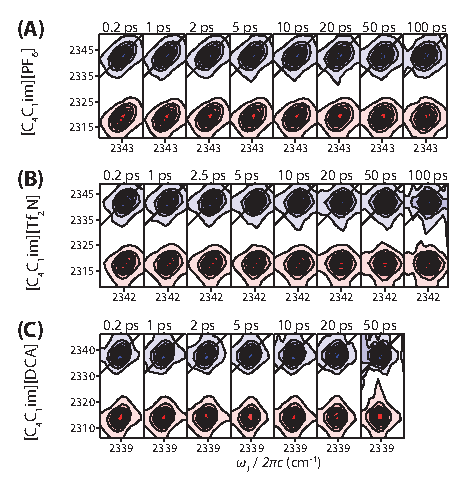
\includegraphics[scale=1.40]{./paper_01/fig7.eps}
  \caption[Experimental 2D-IR spectra of \texorpdfstring{\ce{CO2}}{carbon dioxide} in \ce{[Im_{4,1}][X]}]{Experimental 2D-IR spectra of \ce{CO2} in \ce{[Im_{4,1}]} (A) \ce{[PF6]}, (B) \ce{[Tf2N]}, and (C) [DCA] show the range of timescales for spectral diffusion in \(\nu_3\). Spectral diffusion results from local structural relaxation around \ce{CO2}. Spectral modelling quantifies the timescale of this structural relaxation, and indicates that the timescale varies by up to an order of magnitude between ionic liquid solvents, and that \ce{CO2} dynamics are likely gated by anion dynamics in these ionic liquids. Spectra for \ce{CO2} in other ionic liquids tested can be found in figure~\ref{paper_01:fig:SI_all_2D}.}
  \label{fig:all 2D}
\end{figure}

We used a global fitting algorithm to quantify the rate of spectral diffusion for \(\nu_3\) in each ionic liquid (Figure~\ref{fig:all 2D}). The main peak in the 2D spectrum is sufficiently separated from the shoulders that it can be treated independently. Simulated spectra were calculated using a third-order response function formalism in the semi-impulsive limit. The frequency-fluctuation correlation function
\begin{equation}
  \label{eq:c2}
  c_{2}(t) = \frac{\delta(t)}{T_2} + \Delta^2 \exp \left( -\frac{t}{\tau_c} \right),
\end{equation}
corresponds to a physical system in which \ce{CO2} senses two distinct timescales of motion. Fast motions, in the homogeneous limit, are modeled by first term, which describes a loss of correlation that is too fast to be quantified. In the time domain lineshape function, this leading term describes exponential decay in the ensemble response from dephasing, (with time constant \(T_2\)); the resulting lineshape in frequency space is a Lorentzian with FWHM of \(\left( \pi T_{2} \right)^{-1}\).

The second term corresponds to processes in the spectral diffusion regime, which create a Kubo lineshape. In the slow modulation limit (where \(\tau_c \Delta \gg 1\)), correlations do not change over the timescale of the molecular response. The resulting lineshape function describes a time-domain Gaussian with a variance of \(\Delta^{-2}\); the corresponding lineshape in frequency space is a Gaussian with FWHM of \(2.355\Delta\).

The analytical lineshape function:
\begin{equation}
  \label{eq:g(t)}
  g(t) = \frac{t}{T_2} + \Delta^2\tau_c^2 \left[ \exp{\left( -\frac{t}{\tau_c} \right)}
	+ \frac{t}{\tau_c} - 1 \right],
\end{equation}
can be used to calculate 2D spectra. Normalization of spectra before fitting removes any contribution from vibrational or orientational relaxation, which we do not model. A constrained nonlinear optimization algorithm globally fits the calculated spectra to experimental spectra by minimizing the sum of squares difference between the data and calculation. The algorithm optimizes \(T_2\), \(\tau_c\), and \(\Delta\), in addition to the central frequency, anharmonicity, the $|00^01{\rangle} \rightarrow |00^02{\rangle}$ transition dipole moment, and the phase. The resulting spectral diffusion time, \(\tau_c\), shows good agreement with that obtained by center line slope (CLS) analysis (section~\ref{anionSI_CLS}).

Experimental and optimized calculated spectra agree in terms of overall lineshape and rate of spectral diffusion (Figure~\ref{fig:TFA 2D fit}). The resulting lineshape parameters can then be used as input for spectral modelling that treats the shoulders and cross-peaks of the spectrum (Section~\ref{sec:shoulders_modeling}).

\begin{figure}
  \centering
  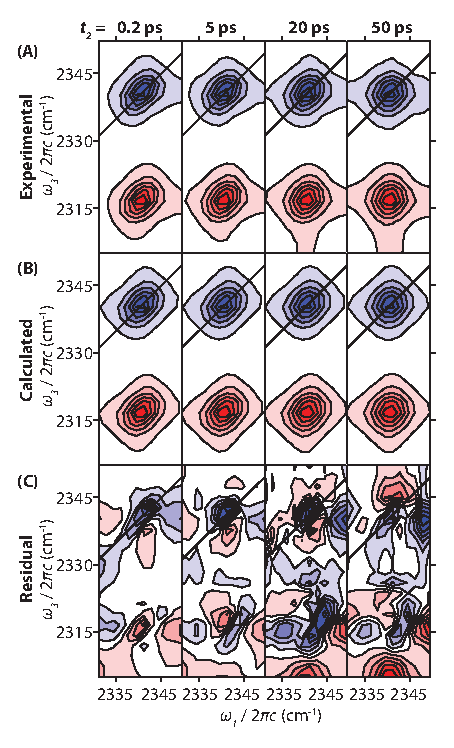
\includegraphics[scale=1.25]{./paper_01/fig8.eps}
  \caption[Example of global fitting of 2D-IR spectra]{\label{fig:TFA 2D fit}Example of global fitting of spectra. (A) Experimental 2D-IR spectra of \ce{CO2} in \ce{[Im_{4,1}]}[TFA]. (B) Calculated 2D-IR for \(\nu_3\) based on a third-order response function, which is fitted to A by optimizing the correlation time \(\tau_c\), frequency range \(\Delta\), and dephasing time \(T_2\), in addition to several other parameters (see text). (C) Residual between the experimental and calculated spectra.}
\end{figure}

\begin{table}
  \centering
  \caption[Best fit correlation function parameters, by ionic liquid]{\label{tab:2}Best fit correlation function parameters, by ionic liquid. \(\tau_c\) indicates the timescale of structural relaxation around \ce{CO2}, the inhomogeneous linewidth \(\Delta\) reflects the range of frequencies experienced by \ce{CO2} in different local environments of each ionic liquid, and the homogeneous dephasing time \(T_2\) arises from fast motions, such as librations, of \ce{CO2}.}
  \begin{tabular}{ccccc}
	\toprule
    Anion & \(\Delta\) (\si{\wavenumber}) & \(\tau_c\) (\si{\ps}) & \(T_2\) (\si{\ps}) \\
    \midrule %TODO fix math
    \ce{[PF6]-} & $2.0 \pm 0.1$ &  $104 \pm 10$ & $3.3 \pm 0.1$ \\
    \ce{[Tf2N]-} & $1.6 \pm 0.1$ &  $26 \pm 5$ & $2.8 \pm 0.1$ \\
    \ce{[TfO]-} & $1.7 \pm 0.1$ & $25 \pm 5$  &  $2.7 \pm 0.1$ \\
    \ce{[TFA]-} & $1.8 \pm 0.1$ & $40 \pm 5$ & $2.6 \pm 0.1$ \\
    \ce{[DCA]-} & $1.6 \pm 0.1$ & $13 \pm 3$ & $3.2 \pm 0.2$ \\
    \ce{[SCN]-} & $1.8 \pm 0.1$ & $16 \pm 3$ & $3.4\pm 0.1$ \\
    \bottomrule
  \end{tabular}
\end{table}

The lineshape parameters (Table~\ref{tab:2}) for \(\nu_3\), combined with insights from computational modeling of \ce{CO2}-anion-cation clusters, help to refine a physical picture of the solvation environment of \ce{CO2} in ionic liquids. The timescale of frequency fluctuation correlations (\(\tau_c\)) for \ce{CO2} varies by up to an order of magnitude between the solvents, from \SI{13(3)}{\ps} in \ce{[Im_{4,1}]}[DCA] to \SI{104(10)}{\ps} in \ce{[Im_{4,1}]}[\ce{PF6}]. The inhomogeneous width (\(\Delta\)) which is largest in \ce{PF6-} and smallest in \ce{DCA-} reflects the diversity of local environments reported by \ce{CO2} in an ionic liquid. The dephasing time (\(T_2\)), which varies from \SIrange{2.6}{3.4}{\ps}, is longer than typical dephasing times in molecular solvents.

A quantitative analysis based on lineshape theory has allowed us to determine the dynamical timescales, dephasing times, and inhomogeneous linewidths for \(\nu_3\) in the six ionic liquids studied.

\subsection{Modelling of Shoulders and Cross-Peaks}
\label{sec:shoulders_modeling}

Having quantified the change in shape of the main 2D \(\nu_3\) band, we now turn to modelling of the dynamics encoded in the diagonal shoulders and cross-peaks.

Fluctuations in the \ce{CO2} \(\nu_2\) population can be described by a thermal equilibrium between \(n\) bending modes:

\begin{equation}
  \label{eq:kinetic}
  |00^00 \rangle \overset{k_{f}}{\underset{k_{r}}\rightleftharpoons} |01^10 \rangle \cdots \overset{k''_{f}}{\underset{k''_{r}}\rightleftharpoons} |0n^l0 \rangle
\end{equation}
The rate of transition between the ground and first excited state, \(k_f\), combined with the Boltzmann distribution of states, determines the remaining rates. \(k_f\) is ultimately determined by the probability of stochastically gain a quantum of energy in a \ce{CO2} bending mode, most likely through collisions in the local environment. The first backwards rate, $k_r$, is directly analogous to the off-equilibrium vibrational energy relaxation rate.

A model that combines probabilistic fluctuations in bending mode population based on Equation \ref{eq:kinetic} with standard response function treatment is able to capture the essential physics required for such stochastic hot bands and their cross-peaks. The frequency of the \(\nu_3\) mode has two sources of variation: (1) the classical bath of intermolecular modes usually encountered in solvation dynamics and (2) the quantum bath of intramolecular vibrations to which the \(\nu_3\) band is coupled. The frequency of the \(\nu_3\) mode, $\omega(t)$ fluctuates as
\begin{equation}
  \label{eq:stochastic_frequency}
  \omega(t) = \braket{\omega} + \delta\omega_\mathrm{inter}(t) + \delta\omega_\mathrm{intra}(t).
\end{equation}
This stochastic frequency can be used as an input to standard nonlinear response function formalism. For example, the first order response function
\begin{equation}
  \label{eq:R1_1}
  R^{(1)}(t) \propto \exp{\left( -i\braket{\omega} t \right)} \times \Braket{ \exp{\left(-i\int_0^t \mathrm{d}t' \delta\omega_\mathrm{inter}(t') + \delta\omega_\mathrm{intra}(t')\right)} },
\end{equation}
can be separated into the two parts, assuming the intra- and inter-molecular modes are uncorrelated,
\begin{equation}\label{eq:R1_2}
  R^{(1)}(t) \propto \exp{\left( -i \braket{\omega} t \right)} \times \Braket{ \exp{\left( -i\int_0^t \mathrm{d}t' \delta\omega_\mathrm{inter}(t') \right)} } \times \Braket{  \exp{\left( -i\int_0^t \mathrm{d}t''\delta\omega_\mathrm{intra}(t'') \right)} }.
\end{equation}
The intermolecular component can be treated with the cumulant expansion truncated at second order
\begin{equation}
  \label{eq:R1_2b}
  R^{(1)}(t) \propto \exp{\left( -i \Braket{\omega} {t} - g(t) \right) } \times \Braket{ \exp{ \left( -i\int_0^t \mathrm{d}t''\delta\omega_\mathrm{intra}(t'') \right)} }.
\end{equation}
where \(g(t)\) is the lineshape function. The extension to third-order response functions is straightforward.

We performed a stochastic simulation in which an ensemble of trajectories was generated by allowing probabilistic instantaneous transitions between the ground and excited states of the \(\nu_2\), with upward and downward rates consistent with the equilibrium populations. These transitions were allowed to happen at any point in the simulation, including during the coherence times.

The simulated lineshape is sensitive to the rate of thermal fluctuations in \(\nu_2\). By tuning the rate constant \(k_f\) of stochastic fluctuation from the ground state into the first excited state and enforcing detailed balance to preserve equilibrium, we can control (1) whether or not diagonal shoulders will appear, and (2) the kinetics of cross-peak formation. In the limit of fast fluctuations, there are no clearly observed shoulders or cross-peaks, as all three peaks coalesce into a single band. In the limit of slow fluctuations, there are clearly defined shoulders, which persist throughout the experimental timescale, and cross-peaks do not grow into the spectrum. In an intermediate regime, we are able to reproduce both the lineshape and kinetics (Figures~\ref{fig:sim spect} and \ref{fig:shoulder kinetics}) seen in the relative intensities of the first shoulder and the cross-peaks between it and the main peak  as functions of population time.

\begin{figure}
  \centering
  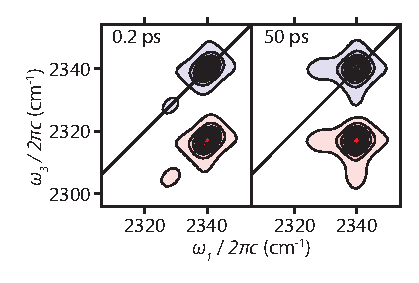
\includegraphics[scale=1.10]{./paper_01/fig9.eps}
  \caption[Stochastic simulation spectrum]{\label{fig:sim spect}Calculated spectrum of \ce{CO2} in \ce{[Im_{4,1}]}[TFA] at $t_2 =$ \SIlist[list-units = single]{0.2;50}{\ps}. Spectra are based on a stochastic simulation that allows the bending mode of a particular oscillator to fluctuate over the course of the experiment (while preserving a Boltzmann distribution). The lineshape as a function of \(t_2\) closely approximates the lineshape of the main peak (1a and 2a), first diagonal shoulder (1b and 2b), and cross-peaks (1b,a; 2a,b and 2b,a) in the experimental spectra (Figure~{\ref{fig:example 2D}}).}
\end{figure}

The microscopic rate constant ($k_{\mathrm{up}}$) for \ce{CO2} bending mode fluctuations in \ce{[Im_{4,1}][TfO]}, from the Monte Carlo simulations is estimated to be $k_{\mathrm{up}} =$ \SI{2.5(1)}{\per\ns}. The corresponding down rate, which is analogous to the vibrational relaxation rate in off-equilibrium pump-probe experiments, is estimated to be $k_{\mathrm{down}} =$\SI{30(12)}{\per\ns}. The kinetic Monte Carlo simulations include the non-equilibrium pumping that was explained by Fayer et al. \cite{Giammanco2016}. Their pump-probe measurements showed an increase in the ground state bleach band due to differences in transition dipole moment between the ground state $|000\rangle$ and the `hot' band $|01^10\rangle$ transition dipole moments. The 2D measurement resolves the excitation frequency, so those dynamics are visible as a separate cross-peaks, where the pump-probe measurement observes the sum of the two peaks (the projection of the spectrum onto the \(\omega_3\)-axis). The main ground state bleach decays with bending mode exchange and the cross-peak grows. If the dipoles of the two states are the same these two terms cancel in the pump-probe measurement; however, the differences in dipole lead to effective rises in the pump-probe ground state bleach signal.

\section{\texorpdfstring{\caps{Molecular Interpretation}}{Molecular Interpretation}}
\label{sec:anions_interpretation}

The resulting molecular picture is that the slower dynamics of the ionic liquid solvent \textit{gate} \ce{CO2}'s dynamics in solution. The slow timescale (\(\tau_c\)) arises from structural relaxation of the solvent around \ce{CO2}, and corresponds to the breakup of local ion shells. Until this liberating event, \ce{CO2} is caged in a relatively well-ordered local environment. Librational and other fast motions only sample a narrow range of instantaneous frequencies, but the variation in instantaneous frequency between different local environments gives rise to the inhomogeneous linewidth.

We assign the inhomogeneous width, \(\Delta\), to the interactions of the \ce{CO2} with its local ion cage. Because charge transfer drives the distortion of the \ce{CO2} geometry, and the geometry determines the \(\nu_3\) frequency, \(\Delta\) reports the range of local structural motifs that the \ce{CO2} can sample.
This range varies from \SI{2}{\wavenumber} in \ce{[PF6]} to \SI{1.6}{\wavenumber} in [DCA]  (a 20\% decrease). \(\Delta\) is also not strongly correlated to the average frequency shift or other structural parameters, and so we attribute it to the range of structures in the condensed phase.

The inhomogeneous linewidth of \ce{CO2} is the narrowest of the IR probes in recent 2D-IR experiments. Thiocyanate, \ce{SCN-}, has a total inhomogeneous linewidth \(\Delta_\mathrm{total} \sim \SI{8}{\wavenumber}\);\cite{Ren2014} heavy water, HOD, \(\Delta_\mathrm{total} \sim \SI{5}{\wavenumber}\);~\cite{wongJPCB-13} and \ce{CO2} \(\Delta_\mathrm{total} \sim \SI{2}{\wavenumber}\). This trend reflects the strength of the coupling of the vibrational chromophore to its environment. The \ce{SCN-} anion is directly integrated into the ion network and hydrogen-bonded to the imidazolium cation through the 2-position. HOD interacts more weakly with the ionic liquid. It associates primarily with the anion, but it is sensitive to the electric field projected on the OH (or OD) bond axis. Because HOD is dipolar, it still experiences relatively large frequency fluctuations. \ce{CO2} is even more weakly still coupled to its environment. \ce{CO2}, which has a quadrupole moment and no dipole moment, is even less influenced by the local electric fields and is sensitive to the more chemical nature of the \ce{CO2}-anion-cation interaction.

Similarly, we assign the spectral diffusion time, \(\tau_c\), to a local ion cage's lifetime around \ce{CO2}. The observed timescale reflects the time for the ion cage around \ce{CO2} to break up and permit \ce{CO2} to move to a novel local environment. This interpretation is consistent with previous computational work which indicate that the ionic liquid solvent reorients spontaneously to accommodate \ce{CO2} in well-defined locations in the ionic liquid,~\cite{Huang2005} and with NMR studies showing a well-defined angular distribution of \ce{CO2} around the cation.~\cite{Corvo2013}

The bulk viscosity, \(\eta\), serves as a proxy for this rate of diffusion which we can compare across the anions. Of course, small, neutral molecules like \ce{CO2} experience less friction from the solvent than the viscosity implies.\cite{Kaintz2013,Kaintz2014-corr} Nevertheless, the linear correlation of bulk viscosity and \(\tau_c\) (\(R^2 = 0.82\))  supports our assignment (Figure~\ref{fig:visc correlation}). This correlation further suggests that the motion of the smaller, more mobile \ce{CO2} through the ionic liquid is gated by the motion of the solvent ions.

\begin{figure}
  \centering
  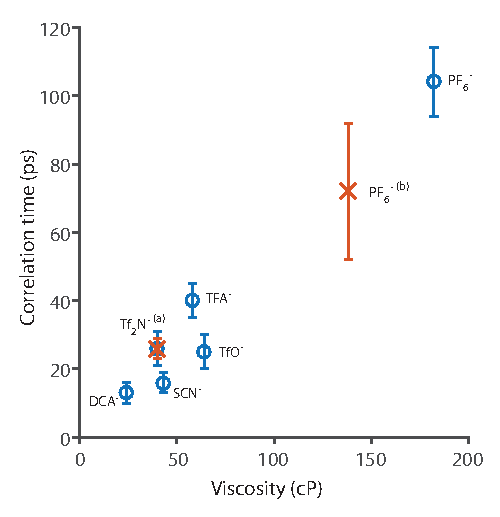
\includegraphics[scale=1.25]{./paper_01/fig10.eps}
  \caption[\texorpdfstring{\(\tau_c\)}{tau(c)}-viscosity correlation with differing ionic liquid anion]{\label{fig:visc correlation}Correlation time, \(\tau_c\), compared with viscosity for the 1-butyl-3-methylimidazolium ionic liquid solvent. Data points marked with an `O' are from \ce{CO2} in this work, while those marked `X' are correlation times from other works (a) \ce{SCN-} in \ce{[Im_{4,1}][Tf2N]},\cite{Ren2014} (b) HOD in \ce{[Im_{4,1}][PF6]},\cite{wongJPCB-13} with ionic liquid viscosity scaled to account for water content.\cite{Li2007}  Literature values for viscosity were used for all ionic liquids.\cite{Tokuda2006a,Domanska2012,Sanchez2009}}
\end{figure}

\ce{CO2} has a Lewis acid-base interaction with the anion of the ionic liquid. Isolated water has possible hydrogen bonds with both the anion and the cation. \ce{SCN-} has a strong electrostatic attraction to the cation. Thus, all three chromophores have different specific interactions with their ionic liquid solvent. Nevertheless, the correlation times seen in 2D-IR studies of \ce{[SCN]-} in \ce{[Im_{4,1}][Tf2N]}\cite{Ren2014} and \ce{D2O}/\ce{HOD} in \ce{[Im_{4,1}][PF6]}\cite{wongJPCB-13} follow the same viscosity trend, when you account for the expected \(\sim 25\)\% decrease in the viscosity of \ce{[Im_{4,1}][PF6]} with \(\chi_{\ce{H2O}} \approx 0.04\).\cite{Li2007} This fact suggests that each of these chromophores is reporting on the local diffusive motion of the surrounding solvent, despite the fact that \ce{SCN-}, water, and \ce{CO2} have different specific interactions with the ions in their solvation shells.

Furthermore, recent MD simulations suggest a direct relationship between ion cage lifetime and bulk transport properties such as self-diffusivity and conductivity.\cite{Zhang2015b} While diffusivity of \ce{CO2} and self-diffusivity of an ionic liquid are not identical parameters, the dynamics reported by \ce{CO2} and \ce{[SCN]-}\cite{Ren2014} in \ce{[Im_{4,1}][Tf2N]} are nearly identical, and both have been related to ion cage lifetime. Thus, it is reasonable to speculate that \ce{CO2} mass transport in these ionic liquids may depend also depend on ion cage lifetime. In this case, the correlation times reported could provide an avenue to directly address the molecular mechanism of \ce{CO2} mass transport in ionic liquids, and might even give insight into other transport properties such as self-diffusivity and conductivity.

The homogeneous dephasing time, \(T_2\), depends on both the timescale of fast motions for \ce{CO2}, $\tau_H$, and on the frequency range experienced during those motions, \(\Delta_H\) ($T_{2} = \left( {\Delta}_H^{2}\tau_H \right)^{-1}$). Experimentally, it is impossible to disentangle these two contributions, but the dephasing time (\(\sim \SI{3}{\ps}\)) is significantly longer than that seen for either HOD (\(\sim \SI{1}{\ps}\)) or \ce{SCN-} (\(\sim \SI{1.4}{\ps}\)) in ionic liquids. Thus, either \ce{CO2} samples a relatively narrow frequency range during its homogeneous motions, or the those motions are particularly fast. Based on the small inhomogeneous linewidth, \(\Delta\), and the fact that \ce{CO2} is a small molecule whose moment of inertia (and consequently, the timescale for fast motions such as librations) is unchanged between ionic liquids and molecular solvents, it seems reasonable that the long dephasing time results from a narrow frequency range in a well-defined local environment, rather than a decrease in solvent interactions that slow the molecule.

Furthermore, the computational results show that, in gas phase clusters, \ce{CO2} bends and adopts a distorted equilibrium geometry. In condensed phase dynamics, transitioning from a linear to a bent geometry could be one method of populating an excited state bending mode, and could have a direct impact on \(k_f\), the rate of bending mode transitions. In principle, the spectral diffusion rate should influence the rate of transition between equilibrium geometries, and thus drive excitation and de-excitation of bending modes. Since we are able to model \(k_f\) based on equilibrium measurements, a systematic study of ionic liquids with different spectral diffusion rates could experimentally elucidate to how the motions of the solvent around a small molecule influence stochastic fluctuations in bending mode population.

These molecular mechanisms can be both tested and clarified by the comparison of these results to simulation. Frequency mapping techniques, combined with classical molecular dynamics simulations can be used to calculate the IR absorption spectrum and the spectral diffusion of modes of interest for small molecules such as water,\cite{steinelCPL-04,Asbury2004,Corcelli2004} nitriles and thiocyanate,\cite{Choi2008,Lindquist2008} and azides\cite{liJPC-06,Li2006} in molecular solvents. More recently these methods have been expanded to explore isolated water in imidazolium ionic liquid solvents\cite{Terranova2014}, with good agreement with experiment.\cite{wongJPCB-13} Similar approaches for \ce{CO2} could verify the molecular mechanism of \ce{CO2} solvation in ionic liquids. It is likely, given the calculated dependence of \(\nu_3\) on \ce{CO2} geometry, that any molecular dynamics simulation would need to account for the geometrical distortion of the \ce{CO2} due to charge transfer, either directly via on-the-fly QM calculations, or with a classical proxy that indirectly accounts for these effects.

These initial studies utilized imidazolium-based ionic liquids because they are commercially available, are ``archetypal,'' and are relatively well-characterized; thus, they provide a good initial platform on which to develop spectroscopic methods. Many ionic liquids of interest, however, involve either novel classes of anions and cations or chemical modification of existing ionic liquids. The changes in solvent structure and dynamics that result from such modifications are generally \textit{not} well-understood. This type of spectroscopy can provide valuable molecular insights into how and why chemical modification of ionic liquids determines bulk properties of interest, especially \ce{CO2} uptake and local ion mobility (which is related to viscosity and conductivity). Chemisorbing ionic liquids are also of interest, especially for carbon capture applications, and many (1) have an initial physisorption step, and (2) have an equilibrium between physisorbed and chemisorbed (reacted) \ce{CO2}. These types of studies could help to elucidate the molecular mechanisms of the equilibrium between \ce{CO2} in its free and bound forms.

\section{\texorpdfstring{\caps{Conclusions}}{Conclusions}}
\label{sec:anions_conclusions}

We have demonstrated that the \ce{CO2} \(\nu_3\) mode can act as a probe of local structure and dynamics in imidazolium ionic liquids. This method has potential application to the analysis of structure and dynamics in ionic liquids being developed for \ce{CO2} capture.

The \(\nu_3\) frequency is sensitive to the timescale of local structural relaxation in ionic liquids. The timescale of this relaxation, \(\tau_c\) is determined by spectral modelling using a third-order response function formalism, with a Bloch-Kubo lineshape. For the imidazolium ionic liquids studied, \(\tau_c\) varies by as much as an order of magnitude between solvents, and correlates with the viscosity of the ionic liquids. The molecular mechanism posited for this timescale is the breakup of local ion cages around the \ce{CO2}.

Computational studies aid understanding the origin of the \(\nu_3\) center frequency shifts in different imidazolium ionic liquids and suggest that geometrical distortion of the \ce{CO2}, driven by charge transfer from the anion into virtual orbitals of \ce{CO2} and from occupied orbitals of \ce{CO2} into virtual orbitals of the cation. A simple one exciton Hamiltonian is able to reproduce the scaled harmonic frequencies with an RMS error of \SI{1.2}{\wavenumber} by accounting for dependence of average frequency, \(\alpha\), on total bond length, \(L\), and the coupling constant, \(\beta\), on magnitude of the angular distortion of \ce{CO2}, \(\theta\).

Anharmonic coupling of \(\nu_2\) and \(\nu_3\) allows thermal fluctuations of \(\nu_2\) population to stochastically shift the \ce{CO2} \(\nu_3\) by units of \SI{-12}{\wavenumber} (the coupling constant), and cause the appearance of a shoulder and dynamic cross-peaks on the 2D spectrum. Modelling of the stochastic bending mode population over the timescale of the experiment gives an estimate of the rate of excitation and de-excitation of bending mode population in the condensed phase at thermal equilibrium, estimated to be \(k_{f} = \SI{2.5 \pm 1}{\per\ns}\) and $k_r = 30\pm12$~\si{\per\ns}. Additional spectral features (the ``second shoulder'' and apparent ``cross-peak'' 1c) arise from fifth-order signal.

The molecular picture that arises from this work is one in which imidazolium ionic liquids solvate \ce{CO2} in well-defined local environments. The interactions of \ce{CO2} with its solvent are dominated by local interactions with its nearest neighbor anion and cation. The picosecond dynamics of \ce{CO2} are gated by the slower local diffusive motions of the anion and cation, whose translations and rotations are hindered due to electrostatic friction from surrounding ions, and potentially due to dispersive interactions between nanosegregated alkyl chains.

The methods and analysis developed in this work describe \ce{CO2} in imidazolium ionic liquids. We expect that they will be transferable, however, to broad classes of materials, such as polymers or metal-organic frameworks, as well as to other ionic liquids.

\section{\texorpdfstring{\caps{Supporting Information}}{Supporting Information}}
\label{paper_01:sec:SI}

\subsection{Comparison of Global Fitting with Center Line Slope}
\label{anionSI_CLS}

For the center line slope method, we fit the signal size as a function of final frequency (\(\omega_3\)) with two Gaussians with opposite signs for each initial frequency (\(\omega_1\)) data point. The resolved positions of the Gaussians of the 0 to 1 transition peak are considered the center points. The center line slope is determined by  fitting the center points linearly as a function of \(\omega_1\). Estimated errors are propagated accordingly.

The resulting center line slope is fitted to a biexponential decay as a function of \(t_2\)
\begin{equation}
c_2 = \sum_{i=1}^2 a_i \exp{\left( -t_2/\tau_i \right)}
\end{equation}
with the resulting parameters for \ce{CO2} \(\nu_3\) in \ce{[Im_{4,1}][TFA]}: \(a = 0.09 \pm 0.04, \tau_1 = 2.1 \pm 2.1 \si{\ps}, b = 0.35 \pm 0.04, \tau_2 = 35 \pm 5 \si{\ps}\).

\begin{figure}[h]
  \centering
  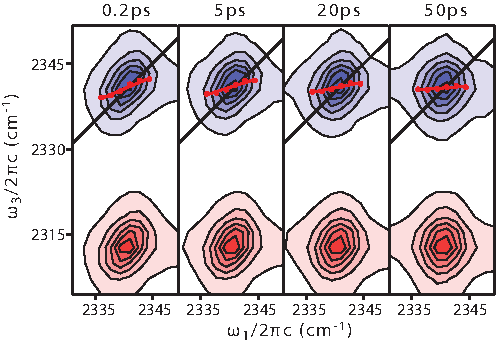
\includegraphics[scale=0.8]{./paper_01/CLS_BMIMTFA.pdf}
  \caption[CLS overlaid on 2D-IR spectrum]{CLS overlaid on the 2D spectrum of \ce{CO2} in \ce{[Im_{4,1}][TFA]}}
\end{figure}

\begin{figure}[h]
  \centering
  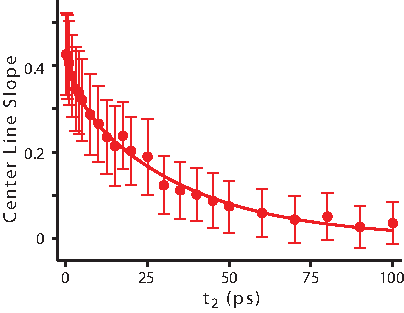
\includegraphics[scale=1]{./paper_01/CLS_fit_BMIMTFA.pdf}
  \caption[CLS fitting of 2D-IR spectrum]{CLS fitting of \ce{CO2} \(\nu_3\) 2D spectrum from \ce{[Im_{4,1}][TFA]}}
\end{figure}

\subsection{2D IR Spectra}
\label{anionSI_2D}

\begin{figure}[h]
  \centering
  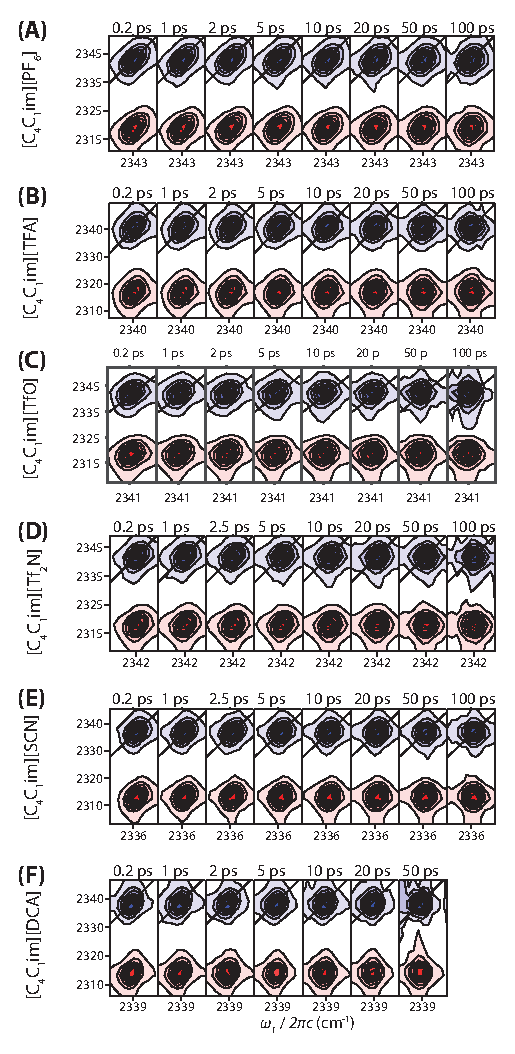
\includegraphics[scale=1.0]{./paper_01/all_2d.eps}
  \caption[Experimental 2D-IR spectra of \texorpdfstring{\ce{CO2}}{carbon dioxide} in all \ce{[Im_{4,1}][X]}]{2D-IR spectra of \ce{CO2} \(\nu_3\) in \ce{[Im_{4,1}+]} (A) \ce{[PF6]-}, (B) \ce{[TFA]-}, (C) \ce{[TfO]-}, (D) \ce{[Tf2N]-}, (E) \ce{[SCN]-}, and (F) \ce{[DCA]-}, showing the range of timescales for spectral diffusion in \(\nu_3\).}
  \label{paper_01:fig:SI_all_2D}
\end{figure}

\subsection{Computational Results}
\label{anionSI_comp}
%Geometries optimized disallowing charge transfer.
In tables~\ref{paper_01:tab:S1}~and~\ref{paper_01:tab:S2}, `\(\nu_1\)' is the frequency of the symmetric stretching mode of \ce{CO2}, and `\(\nu_3\)' is the frequency of the antisymmetric stretching mode of \ce{CO2}. \(\alpha\) is the average of the two normal mode frequencies, \(\alpha = (\omega_\mathrm{s} + \omega_\mathrm{a})/2\). \(\beta\) is the coupling constant, or the difference of the two local mode frequencies, \(\beta = (\omega_\mathrm{s} - \omega_\mathrm{a})/2\).

`CT: \ce{CO2} to IL` is the amount of charge transferred from the \ce{CO2} into the ionic liquid components, `CT: IL to \ce{CO2}` is the amount of charge transferred from the ionic liquid components into the \ce{CO2}, and `CT: net` is the net charge transferred into the \ce{CO2}.

`geom: angle' is the \ce{CO2} \ce{O--C--O} angle, and `geom: \(\theta\)' is the deviation of the angle from \ang{180}. `geom: \(l_1\)' and `geom: \(l_2\)' are the bond lengths of the two \ce{C-O} bonds, `geom: \(l_2 - l_1\)' is the difference between the two bonds lengths, and `geom: \(L\)` is the sum of the two bond lengths. `geom: \ce{O_{12}}' is the through-space oxygen-oxygen distance in \ce{CO2}.

\begin{landscape}
  \begin{table}
    \centering
    % \resizebox{1\textwidth}{!}{
    \caption{\texorpdfstring{\cotil}{Carbon dioxide-IL} geometries optimized allowing charge transfer}
    \label{paper_01:tab:S1}
    \small
    \tabcolsep=0.11cm
    \begin{tabular}{rcccccccccc}
      \hline
      & Free \ce{CO2} & Cation & \ce{BF4} & \ce{DCA} & \ce{PF6} & \ce{SCN} & \ce{TFA} & \ce{Tf2N} & \ce{TfO} \\
      \hline
      \(\nu_1\) (\si{\wavenumber}) & 1371.93 & 1372.12 & 1372.96 & 1370.71 & 1373.95 & 1370.35 & 1371.68 & 1372.88 & 1371.14 \\
      \(\nu_3\) (\si{\wavenumber}) & 2436.1 & 2443.07 & 2434.71 & 2430.85 & 2437.48 & 2430.27 & 2429.81 & 2437.74 & 2433.89 \\
      \(\beta\) (\si{\wavenumber}) & -532.085 & -535.475 & -530.875 & -530.07 & -531.765 & -529.96 & -529.065 & -532.43 & -531.375 \\
      \(\alpha\) (\si{\wavenumber}) & 1904.015 & 1907.595 & 1903.835 & 1900.7 & 1905.715 & 1900.31 & 1900.745 & 1905.31 & 1902.515 \\
      \hline
      CT: \ce{CO2} to IL (\si{\milli\elementarycharge}) & 0 & 2.251 & 1.264 & 2.259 & 1.012 & 1.323 & 1.618 & 1.603 & 2.339 \\
      CT: IL to \ce{CO2} (\si{\milli\elementarycharge}) & 0 & 0.079 & 4.558 & 3.376 & 3.336 & 3.317 & 5.131 & 2.493 & 3.009 \\
      CT: net (\si{\milli\elementarycharge}) & 0 & -2.172 & 3.294 & 1.117 & 2.324 & 1.994 & 3.513 & 0.89 & 0.67 \\
      \hline
      geom: angle (\si{\degree}) & 179.96 & 179.93 & 175.49 & 175.01 & 176.21 & 175.65 & 174.78 & 177.36 & 175.99 \\
      geom: \(\theta\) (\si{\degree}) & 0.042 & 0.07 & 4.51 & 4.99 & 3.79 & 4.35 & 5.22 & 2.64 & 4.01 \\
      geom: \(l_2 - l_1\) (\si{\angstrom}) & \num{1.9e-7} & 0.015 & 0.0087 & 0.011 & 0.0071 & 0.0089 & 0.0076 & 0.0076 & 0.011 \\
      geom: \(l_1\) (\si{\angstrom}) & 1.169 & 1.176 & 1.174 & 1.175 & 1.173 & 1.165 & 1.173 & 1.165 & 1.175 \\
      geom: \(l_2\) (\si{\angstrom}) & 1.169 & 1.161 & 1.165 & 1.164 & 1.165 & 1.174 & 1.166 & 1.173 & 1.164 \\
      geom: \ce{O_{12}}  (\si{\angstrom}) & 2.338 & 2.337 & 2.337 & 2.337 & 2.337 & 2.338 & 2.337 & 2.337 & 2.337 \\
      geom: \(L\) (\si{\angstrom}) & 2.338 & 2.337 & 2.338 & 2.339 & 2.338 & 2.339 & 2.339 & 2.338 & 2.339 \\
    \end{tabular}%}
    \normalsize
  \end{table}


  \begin{table}
    \centering
    % \resizebox{1\textwidth}{!}{
    \caption{\texorpdfstring{\cotil}{Carbon dioxide-IL} geometries optimized without allowing charge transfer}
    \label{paper_01:tab:S2}
    \small
    \tabcolsep=0.11cm
    \begin{tabular}{rcccccccccc}
      \hline
      & Free \ce{CO2} & Cation & \ce{BF4} & \ce{DCA} & \ce{PF6} & \ce{SCN} & \ce{TFA} & \ce{Tf2N} & \ce{TfO} \\
      \hline
      \(\nu_1\) (\si{\wavenumber}) & 1371.93 & 1371.47 & 1373.31 & 1373.44 & 1373.33 & 1373.14 & 1373.65 & 1373.06 & 1373.45 \\
      \(\nu_3\) (\si{\wavenumber}) & 2436.1 & 2439.86 & 2438.56 & 2439.1 & 2438.47 & 2438.78 & 2438.39 & 2438.767 & 2439.37 \\
      \(\beta\) (\si{\wavenumber}) & -532.085 & -534.195 & -532.625 & -532.83 & -532.57 & -532.82 & -532.37 & -532.85 & -532.96 \\
      \(\alpha\) (\si{\wavenumber}) & 1904.015 & 1905.665 & 1905.935 & 1906.27 & 1905.9 & 1905.96 & 1906.0271905.91 & 1906.41 \\
      \hline
      CT: \ce{CO2} to IL (\si{\milli\elementarycharge}) & 0 & 1.743 & 1.038 & 1.836 & 1.154 & 1.302 & 1.023 & 1.246 & 1.941 \\
      CT: IL to \ce{CO2} (\si{\milli\elementarycharge}) & 0 & 0.039 & 3.053 & 2.266 & 2.221 & 1.64 & 2.916 & 1.274 & 2.048 \\
      CT: net (\si{\milli\elementarycharge}) & 0 & -1.704 & 2.015 & 0.43 & 1.067 & 0.338 & 1.893 & 0.028 & 0.107 \\
      \hline
      geom: angle (\si{\degree}) & 179.96 & 179.97 & 177.30 & 177.29 & 177.58 & 177.78 & 178.30 & 177.19 & 177.39 \\
      geom: \(\theta\) (\si{\degree}) & 0.04 & 0.03 & 2.70 & 2.70 & 2.42 & 2.22 & 1.70 & 2.81 & 2.61 \\
      geom: \(l_2 - l_1\) (\si{\angstrom}) & $1.9\times 10^{-7}$ & 0.012 & 0.008 & 0.008 & 0.007 & 0.008 & 0.007 & 0.007 & 0.009 \\
      geom: \(l_1\) (\si{\angstrom}) & 1.169 & 1.175 & 1.173 & 1.173 & 1.172 & 1.165 & 1.166 & 1.172 & 1.173 \\
      geom: \(l_2\) (\si{\angstrom}) & 1.169 & 1.163 & 1.165 & 1.165 & 1.166 & 1.173 & 1.172 & 1.166 & 1.165 \\
      geom: \ce{O_{12}} (\si{\angstrom}) & 2.338 & 2.338 & 2.337 & 2.337 & 2.337 & 2.337 & 2.338 & 2.337 & 2.337 \\
      geom: \(L\) (\si{\angstrom}) & 2.338 & 2.338 & 2.338 & 2.338 & 2.338 & 2.338 & 2.338 & 2.338 & 2.338 \\
    \end{tabular}%}
    \normalsize
  \end{table}
\end{landscape}
